%% LyX 2.0.6 created this file.  For more info, see http://www.lyx.org/.
%% Do not edit unless you really know what you are doing.
\documentclass[a4paper,american]{book}
\usepackage[T1]{fontenc}
\usepackage[latin9]{inputenc}
\pagestyle{plain}
\setcounter{tocdepth}{3}
\synctex=-1
\usepackage{amssymb}
\usepackage{graphicx}

\makeatletter

%%%%%%%%%%%%%%%%%%%%%%%%%%%%%% LyX specific LaTeX commands.
\pdfpageheight\paperheight
\pdfpagewidth\paperwidth

%% Because html converters don't know tabularnewline
\providecommand{\tabularnewline}{\\}

%%%%%%%%%%%%%%%%%%%%%%%%%%%%%% Textclass specific LaTeX commands.
\newenvironment{lyxcode}
{\par\begin{list}{}{
\setlength{\rightmargin}{\leftmargin}
\setlength{\listparindent}{0pt}% needed for AMS classes
\raggedright
\setlength{\itemsep}{0pt}
\setlength{\parsep}{0pt}
\normalfont\ttfamily}%
 \item[]}
{\end{list}}

%%%%%%%%%%%%%%%%%%%%%%%%%%%%%% User specified LaTeX commands.
\usepackage{wrapfig}
 \setlength{\intextsep}{0cm plus1cm minus1cm}
\newcommand{\menuitem}[1]{\textbf{\emph{#1}}}

\makeatother

\usepackage{babel}
\begin{document}
\begin{flushleft}
\thispagestyle{empty}
\par\end{flushleft}

\vspace{0.2in}


\begin{center}
{\Huge{expEYES }}{\Large{Junior}}
\par\end{center}{\Large \par}

\begin{center}
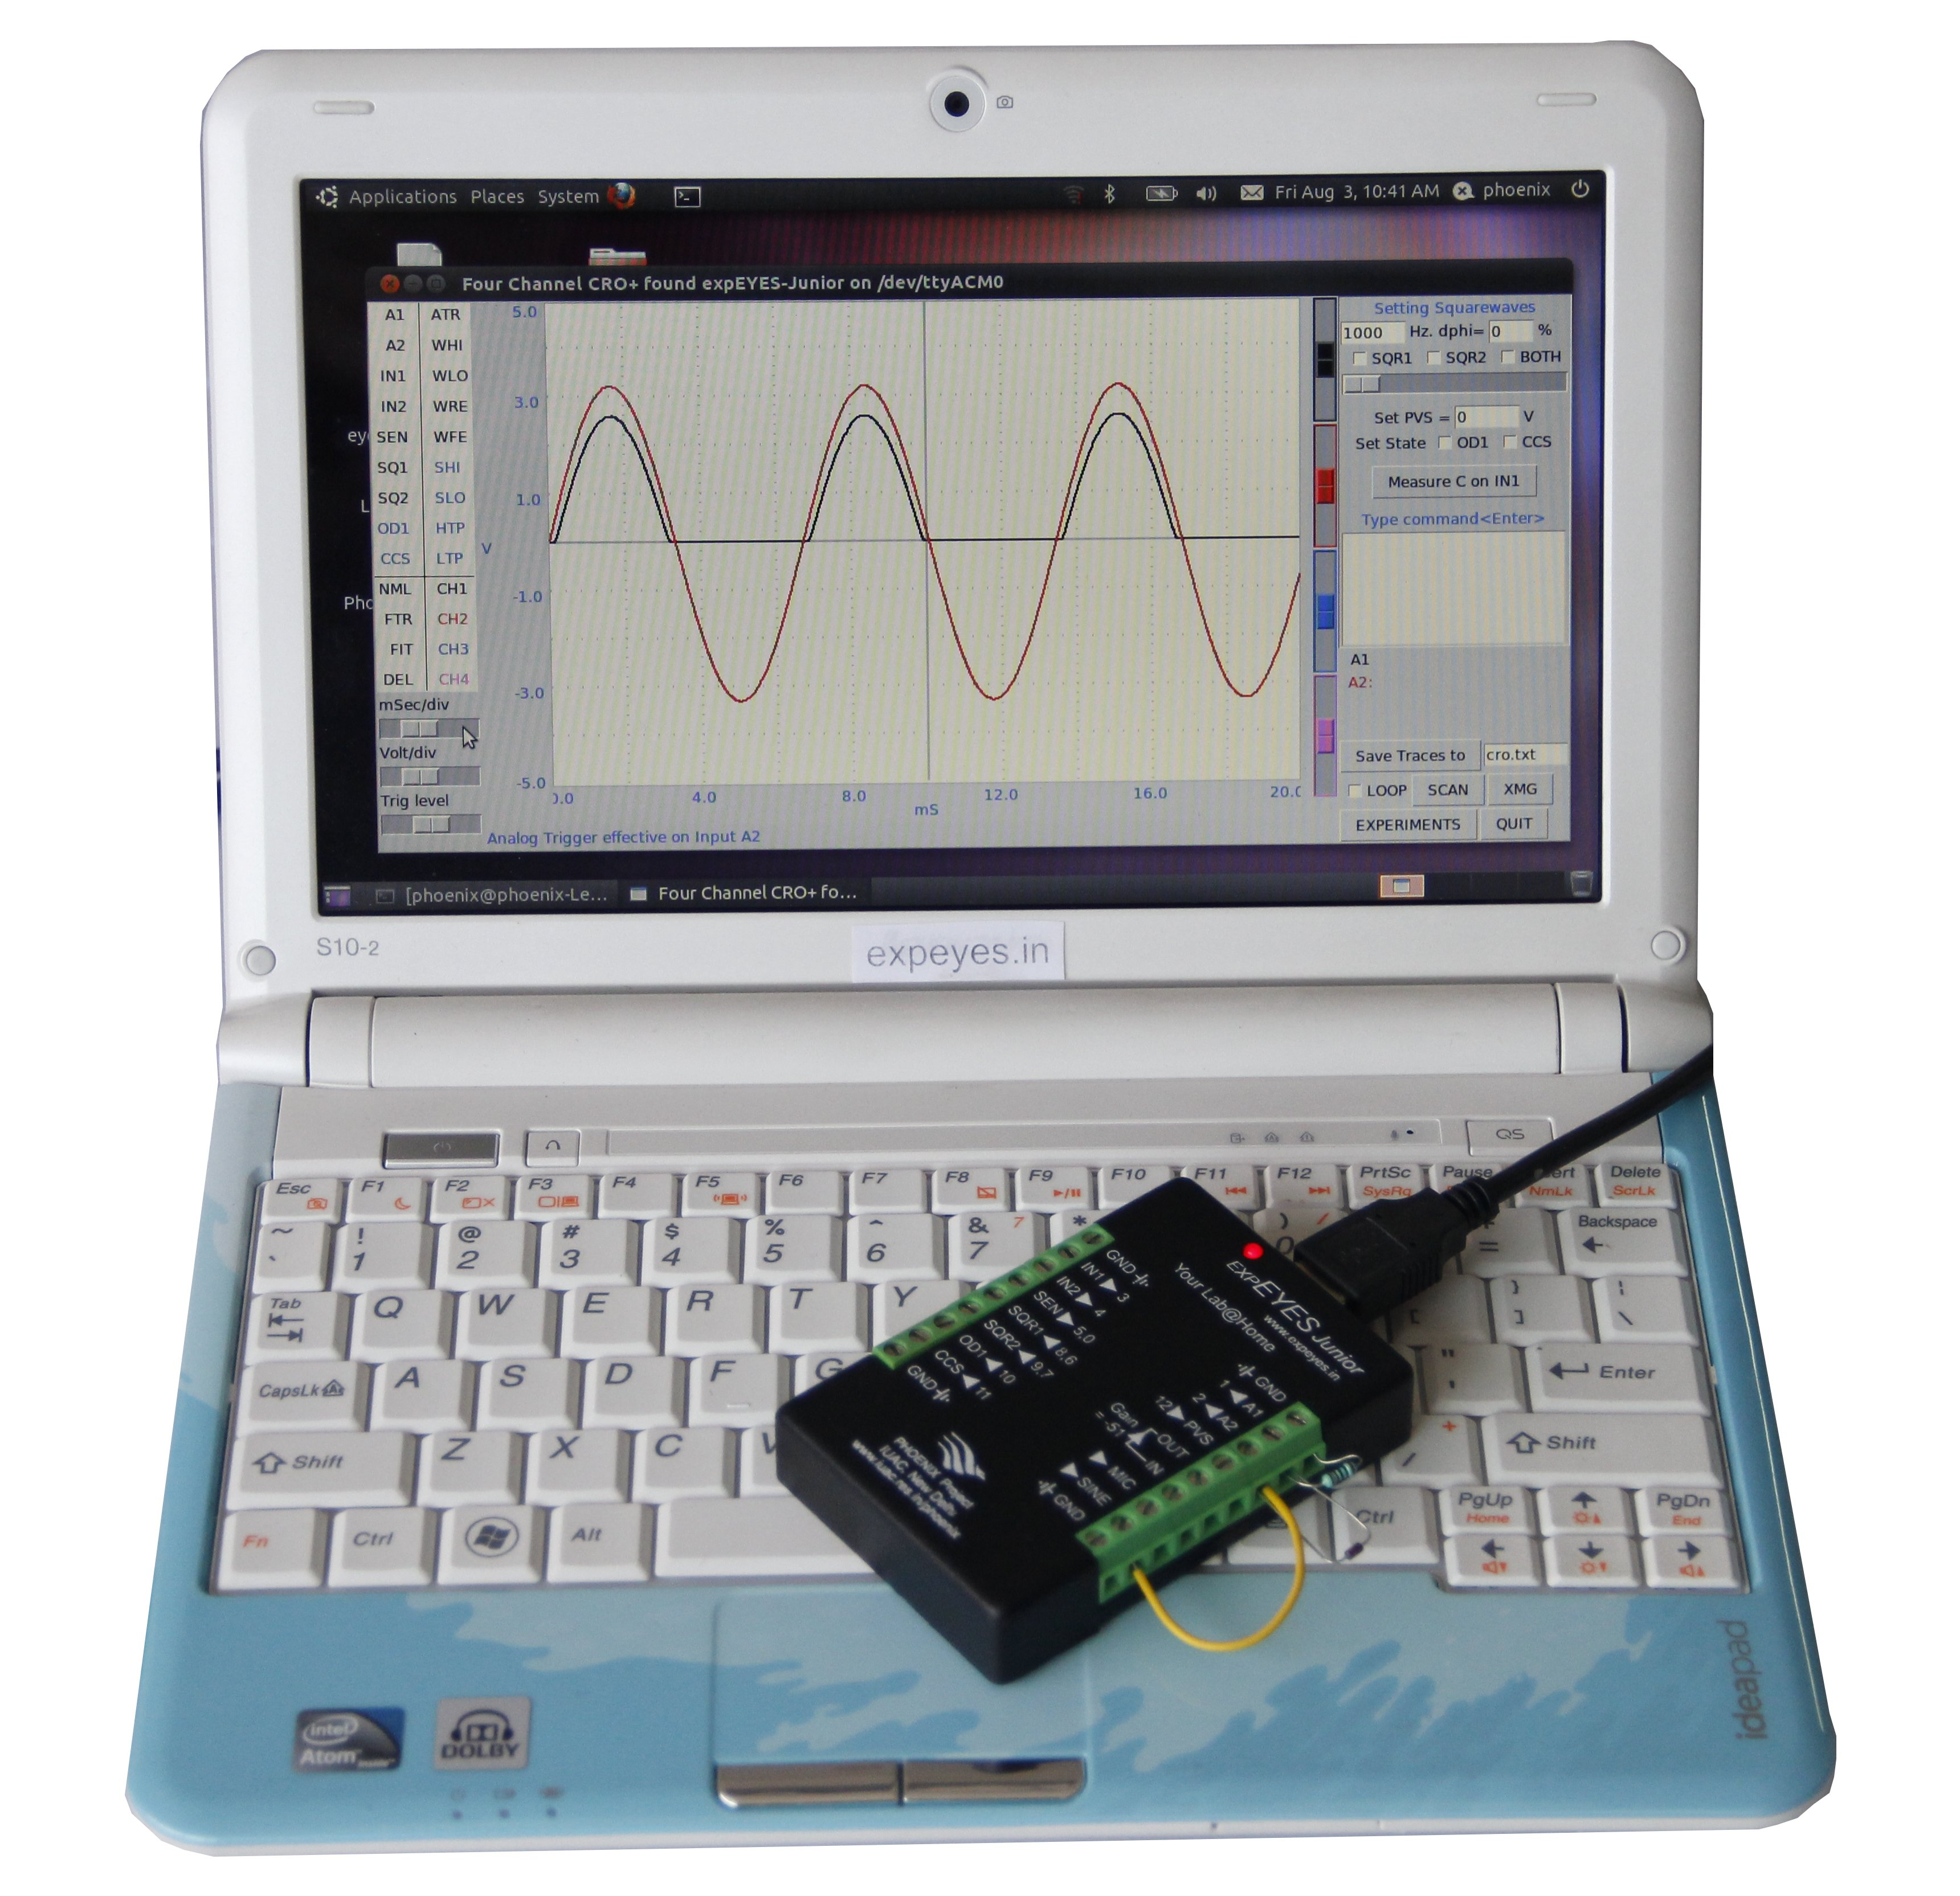
\includegraphics[width=5cm]{pics/ej-with-netbook-hr}
\par\end{center}

\begin{center}
{\large{User's Manual }}
\par\end{center}{\large \par}

\begin{center}
{\LARGE{Experiments for}}\\
{\LARGE{ Young Engineers and Scientists}}
\par\end{center}{\LARGE \par}

\begin{center}
http://expeyes.in
\par\end{center}

\begin{center}
from
\par\end{center}

\begin{center}
PHOENIX Project\\
Inter-University Accelerator Centre \\
(A Research Centre of UGC)\\
New Delhi 110 067\\
www.iuac.res.in
\par\end{center}

\newpage{}

Preface

The PHOENIX (Physics with Home-made Equipment \& Innovative Experiments)
project was started in 2004 by Inter-University Accelerator Centre
with the objective of improving the science education at Indian Universities.
Development of low cost laboratory equipment and training teachers
are the two major activities under this project. 

expEYES Junior is a modified version of expEYES released earlier.
It is meant to be a tool for learning by exploration, suitable for
high school classes and above. We have tried optimizing the design
to be simple, flexible, rugged and low cost. The low price makes it
affordable to individuals and we hope to see students performing experiments
outside the four walls of the laboratory, that closes when the bell
rings.

Hardware design is open and royalty-free. The software is released
under GNU General Public License. The project has progressed due to
the active participation and contributions from the user community
and many other persons outside IUAC. We are thankful to S Venkataramanan
and Prof. R Nagarajan for correcting this document by carrying out
the experiments described independently. 

expEYES Junior user's manual is distributed under GNU Free Documentation
License. For more details about the project visit the website \textit{expeyes.in}

~

Ajith Kumar B.P. ~~~~~~~~~(ajith@iuac.res.in)

V V V Satyanarayana

Jimson Sacharias

\newpage{}

\tableofcontents{}


\chapter{Getting Started}


\section{Introduction }

Science is the study of the physical world by systematic observations
and experiments. Proper science education is essential for cultivating
a society where reasoning and logical thinking prevails and not superstition
and irrational beliefs. Science education is also essential for training
enough technicians, engineers and scientists for the economy of the
modern world. It is widely accepted that personal experience in the
form of experiments and observations, either carried out by students
or performed as demonstrations by teachers, are essential to the pedagogy
of science. However, almost everywhere science is mostly taught from
the text books without giving importance to experiments, partly due
to lack of equipment. As a result, most of the students fail to correlate
their classroom experience to problems encountered in daily life.
To some extent this can be corrected by learning science based on
exploration and experimenting. 

The advent of personal computers and their easy availability has opened
up a new path for making laboratory equipment. Addition of some hardware
to an ordinary computer can convert it in to a science laboratory.
Performing quick measurements with good accuracy enables one to study
a wide range of phenomena. Science experiments generally involve measuring/controlling
physical parameters like temperature, pressure, velocity, acceleration,
force, voltage, current etc. If the measured physical property is
changing rapidly, the measurements need to be automated and a computer
becomes a useful tool. For example, understanding the variation of
AC mains voltage with time requires measuring it after every millisecond.

The ability to perform experiments with reasonable accuracy also opens
up the possibility of research oriented science education. Students
can compare the experimental data with mathematical models and examine
the fundamental laws governing various phenomena. Something similar
to what research scientists do but with less sophisticated equipment.
The expEYES ( expEriments for Young Engineers \& Scientists) kit is
designed to support a wide range of experiments, from school to post
graduate level. It also acts as a test equipment for electronics engineers
and hobbyists. The simple and open architecture of expEYES allows
the users to \textit{develop new experiments, without getting into
the details of electronics or computer programming}. This User's manual
describes \textit{expEYES} Junior along with several experiments,
there is also a Programmer's manual available.


\section{The equipment}

ExpEYES Junior is interfaced and powered by the USB port of the computer.
For connecting external signals, it has several Input/Output terminals,
arranged on both sides, as shown in figure \ref{fig:The-ExpEYES-toppanel}.
It can monitor and control the voltages at these terminals. In order
to measure other parameters (like temperature, pressure etc.), we
need to convert them in to electrical signals by using appropriate
sensor elements. 

Even though our primary objective is to do experiments, you are advised
to read through the brief description of the equipment given below.
The device can be also used as a test equipment for electrical and
electronics engineering experiments.


\paragraph*{\textit{IMPORTANT : }}

\textit{The external voltages connected to expEYES must be within
the allowed limits. Inputs A1 and A2 must be within $\pm5$ volts
range and Inputs IN1 and IN2 must be in 0 to 5V range. Exceeding these
limits slightly will flash an error message. If the program stops
responding, exit and re-connect the USB to reset the device. Larger
voltages will result in permanent damage. To measure higher voltages,
scale them down using resistive potential divider networks.}

\begin{figure}
\begin{centering}
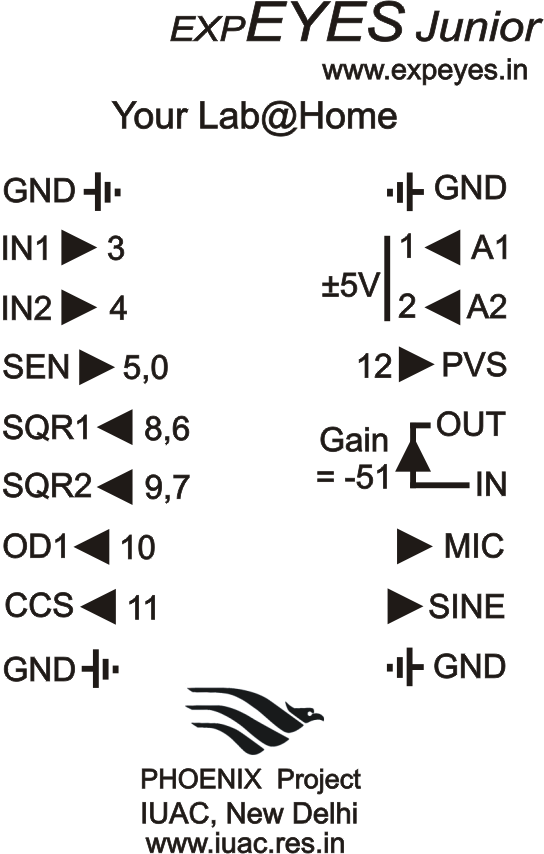
\includegraphics[height=9cm]{pics/top-panel}
\par\end{centering}

\caption{The ExpEYES Junior top panel showing the external connections on both
sides.The channel numbers shown against some terminals are meant for
those who write software to access them. The arrows indicates the
direction of the signals, for example arrow from $A1\Rightarrow1$
means the signal from terminal A1 goes to channel number 1.\label{fig:The-ExpEYES-toppanel}}
\end{figure}



\subsection{External connections}

The functions of the external Input/Outputs terminals are briefly
explained below.


\paragraph*{Programmable Voltage Source (PVS) :}

Can be set, from software, to any value in the 0 to +5V range. The
resolution is 12 bits, implies a minimum voltage step of around 1.25
millivolts. There is a read-back to verify PVS.


\paragraph*{$\pm5V$ Analog Inputs (A1 \& A2) : }

Can measure voltage within the $\pm5$ volts range. The resolution
of ADC used is 12 bits. Voltage at these terminals can be displayed
as a function of time, giving the functionality of a low frequency
oscilloscope. The maximum sampling rate is 250,000 per second. Both
have an input impedance of $10M\Omega$ .


\paragraph*{$0-5V$ Analog Inputs (IN1 \& IN2):}

These terminals can measure voltages in the 0 to 5V range. 


\paragraph*{Resistive Sensor Input (SEN):}

This is mainly meant for sensors like Light Dependent Resistor, Thermistor,
Photo-transistor etc.. SEN is connected to 5 volts through a $5.1k\Omega$
resistor. It also has a built-in analog comparator.


\paragraph*{Digital Inputs (IN1 \& IN2):}

The inputs IN1, IN2 can act as both analog and digital inputs. In
the digital mode, any voltage less than 1 volt is treated as logic
0(LOW) and anything higher than 2.5 volts is treated as logic 1(HIGH).
If the voltage input is changing periodically between HIGH and LOW,
these terminals can measure the frequency and duty-cycle of the connected
signal. Time interval between voltage transitions on these pins can
be measured with microsecond resolution.


\paragraph*{Digital Output (OD1) :}

The voltage at OD1 can be set to 0 or 5 volts, using software.


\paragraph*{Square Waves SQR1 \& SQR2 : }

Output swings from 0 to 5 volts and frequency can be varied 0.7Hz
to 100kHz. All intermediate values of frequency are not possible.
SQR1 and SQR2 can be set to different frequencies. It is also possible
to set them to same frequency, with a specific phase shift between
the two. These outputs also can be programmed to generate Pulse Width
Modulated waveforms. SQR1 is wired to channel 6 for read-back and
SQR2 is wired to channel 7.

Setting frequency to $0$Hz will make the output HIGH and setting
it to $-1$ will make it LOW, in both cases the wave generation is
disabled. When the wave generation is disabled, SQR1 and SQR2 can
act as digital outputs on channel 8 and 9 respectively.

SQR1 output has a\textbf{\textsl{ $100\Omega$ series resistor}} so
that it can drive LEDs directly. 


\paragraph*{Infrared Transmission}

An Infrared Diode connected to SQR1 can transmit data using IR transmission
protocol. The 4 byte transmission can be used for emulating common
TV remotes. It also supports a single byte transmission that can be
received by a program running on a micro-controller%
\footnote{http://expeyes.in/micro-controllers-for-hobby-projects-and-education%
}.


\paragraph*{SINE wave: }

Fixed frequency sine wave generator, frequency is around 150 Hz. Bipolar
signal output with an amplitude of around 4 volts.


\paragraph*{Constant Current Source (CCS) : }

The constant current source can be switched ON and OFF under software
control. The nominal value is 1mA but may vary from unit to unit,
due to component tolerances. To measure the exact value, connect an
ammeter from CCS to GND. Another method is to connect a known resistance
(\textasciitilde{}3.3k) and measure the voltage drop across it. The
load resistor should be less than 4k for this current source.


\paragraph*{Microphone (MIC) :}

There is a built-in condenser microphone (on the side, near CCS).
Its output, amplified 51 times, is available on MIC output. Connect
it to A1 or A2 for viewing.


\paragraph*{Inverting Amplifier (IN->OUT) : }

The inverting amplifier is implemented using TL084 op-amp. Rf=51000
and Ri = 1000, giving a maximum gain of $\frac{51000}{1000}=51$.
The gain can be reduced by feeding the input via a resistor. For example,
using a 50k series resistor will make it a unity gain inverter.


\paragraph*{Ground : }

The four terminals marked as GND are the reference ground. All the
generated/measured voltages are with respect to these terminals.


\subsection{Accessory Set}

Some accessories are provided with expEYES Junior, a photograph is
given on back cover of the manual.
\begin{itemize}
\item Crocodile Clips with leads (4) : If the connection to any terminal
is changed many times during an experiment, it is easier to make the
connection using the crocodile clip provided.
\item 3000 Turns Coil (2) : 44SWG copper wire, Inductance $\approx$ 125
mH, Resistance $\approx$ 550 $\Omega$ . These coils can be used
for studying inductance, electromagnetic induction etc. 
\item Piezo Electric Discs (2) : Resonant frequency is around 3500 Hz. Can
be energized by SQR1 or SQR2. Discs are enclosed in a plastic shell
that forms a cavity, that enhances the amplitude of sound produced.
\item DC Motor : Should be powered by a DC voltage less than 3 volts.
\item Permanent Magnets : (a) 10mm dia \& length (b) 5 mm dia \& 10 mm length
(c) Button size magnets(2)
\item 5mm LEDS : RED, BLUE, GREEN, WHITE
\item Capacitors : 47uF, 1uF, 0.1uF \& 0.01 uF
\item Resistors : 560$\Omega$, 1$k\Omega$, 2.2$k\Omega$ , 10$k\Omega$
, 51$k\Omega$ and 200 $k\Omega$
\item LDR \& Thermistor
\item Two silicon diodes (1N4148) and a Transistor( 2N2222)
\item 5 pieces of wires (8cm) and a Screwdriver 
\end{itemize}

\section{Software Installation}

ExpEYES can run on any computer having a Python Interpreter and a
Python module to access the Serial port. The USB interface is handled
by the device driver program that presents the USB port as an RS232
port to the application programs. The communication the expEYES is
done using a library written in Python language (also available in
C language). Programs with GUI have been written for many experiments.
There are many ways to get the software running:


\subsubsection*{The expEYES Live CD }

The easiest way to get started is to boot your PC with the expEYES
Live-CD. From the PC BIOS, make the CD drive as the first boot device,
insert the live CD and reboot the PC. A desktop will appear and you
can start expEYES Junior from the menu \textbf{Applications->Science}->EYES-Junior.
You can also start it from a Terminal using the command:
\begin{lyxcode}
\$~python~/usr/share/expeyes-junior/croplus.py
\end{lyxcode}

\subsubsection*{Installing on Debian or Ubuntu GNU/Linux distributions}

Download \textbf{expeyes-3.0.0.deb} , or higher version, from the
software section of \textbf{http://expeyes.in} and install it. It
depends on python-serial, python-tk, python-scipy and grace (a 2D
plotting program).


\subsubsection*{For other GNU/Linux distributions}

Download \textbf{expeyes-3.x.x.zip} from \textbf{http://expeyes.in}
and follow the instructions in the README file. It is important to
give read/write permissions for all users on the USB port where expEYES
is connected. This can be done by running the \textit{postint} shell
script, included in the zip file.


\subsubsection*{On MSWindows}

Even though expEYES is Free Software and is developed using Free and
Open software, it runs on non-free platforms also. To install it on
MS windows, you need (1) MCP2200 drivers (2) Python-2.x version, python-serial,
python-tk, python-numpy and python-scipy (3) expeyes-3.x.x.zip

Unzip the file \textbf{expeyes-3.x.x.zip}, and double click on \textbf{croplus.py}
inside the newly created directory named expeyes-3.x.x\textbackslash{}eyes-junior.
If you have expEYES liveCD, browse inside the directory names WINEYES.
All the files mentioned above are inside that directory. Double click
on them in the order mentioned above to install them. See the software
section on the expeyes website for more details.


\section{The main GUI program}

\begin{figure}
\begin{centering}
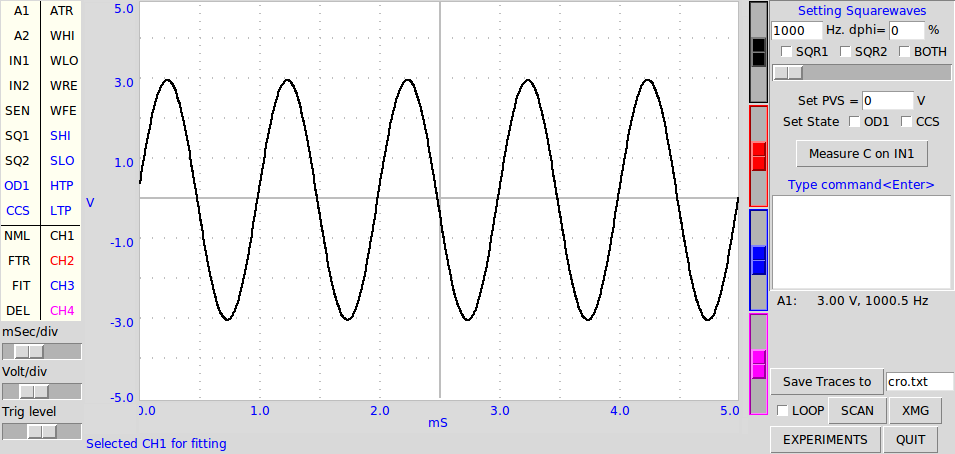
\includegraphics[width=11cm]{pics/benchmark}
\par\end{centering}

\caption{The croplus screen showing a sine-wave connected to A1. \label{fig:The-croplus-screen.}}
\end{figure}


Start Applications->Science->EYES-Junior from the menu. A four channel
oscilloscope screen with several extra features will open as shown
in figure \ref{fig:The-croplus-screen.}. The \textit{\menuitem{EXPERIMENTS}
}button pops up a menu of programs for several experiments. The main
window will become inactive when an experiment is selected and running.


\subsubsection*{The Plot Window}

The plot window works like a low frequency four channel oscilloscope.
The maximum sampling rate is 250 kHz only, sufficient for exploring
audio frequency range. A brief description of this GUI program is
given below.
\begin{itemize}
\item On the left side, the Inputs (A1,A2,IN1,IN2,SEN and read backs of
SQR1 \& SQR2) are shown. \textit{Clicking on any of them will display
the voltage/logic level present. }To plot any of them, drag it to
the desired channel (CH1 to CH4). The names of inputs selected for
display are shown on the right side of the plot window, using a unique
color for each channel.
\item For online help, place cursor on any item, press and hold the left
mouse button.
\item Dragging ATR to any of the inputs will make it the CRO trigger source.
\item This program allows different types of triggering. For example, dragging
WRE to IN1 will enable rising edge triggering on it. It also supports
setting levels or generating pulses on Digital outputs just before
capturing the waveform. Dragging SHI to OD1 will keep OD1 HIGH during
the capture process. For more details refer to the programmers manual.
\item Dragging any of the channels, CH1 to CH4, to FIT will enable calculating
amplitude and frequency by fitting the data using the equation $V=V_{0}\sin\left(2\pi ft+\theta\right)+C$
, $V_{0}$ and $f$ will be displayed. Dragging the channel to NML
will disable the FIT option.
\item Right clicking on IN1, IN2, SEN, SQR1 or SQR2 will measure the frequency
and duty cycle of the voltage waveform present at the terminal.
\item If two adjacent channels are assigned, Right-clicking on the first
will calculate frequency and phase difference between the two inputs.
\item Dragging a channel to FTR will show the Fourier Spectrum of the waveform
in a separate window.
\item To remove a displayed input, drag it to DEL.
\item Horizontal scale (ms/division) adjustment. Set this to the minimum
value and increase to view more number of cycles on the screen. Drag
the rider or click on the left/right sides of it.
\item Vertical scale (volts/division). Maximum values is 5 volts per division.
\item Vertical offset sliders are provided for each channel to shift the
trace up or down.
\item The Check button LOOP selects Single/Continuous mode of scanning.
\item The traces can be transferred to an Grace plot window, using XMG.
\item SAVE button to save the data to the specified file in\textit{ }two
column text format.
\end{itemize}
In addition to the CRO features, you can also control SQR1, SQR2,
PVS etc. from the GUI. You can execute Python functions to access
the hardware from a command window.
\begin{itemize}
\item For the Square waves , the frequency and phase difference in percentage
are entered in two text fields. SQR1 \& SQR2 can be set to different
frequencies or to a single frequency with desired phase difference.
Re-activate the check buttons after changing frequency or phase difference. 
\item SQR1 can be set using a slider also.
\item To Set PVS, type the voltage (0 to 5) and press Enter key. The PVS
output has a readback and the read back value is displayed in the
message field.
\item Checkbuttons are provided to control OD1 and CCS.
\item Capacitance connected between IN1 and GND can be measured.
\item Python functions to communicate to the hardware can be entered in
a Command Window.
\end{itemize}

\section{Basic measurements using expEYES}

Before proceeding with the experiments, let us do some simple exercises
to become familiar with expEYES Junior. Boot your computer from the
LiveCD, connect the device a USB port and start the EYES-Junior program
from the menu 'Applications->Science'.


\subsection{Generate \& measure voltages}
\begin{itemize}
\item Connect PVS to IN1 and Assign IN1 to CH1
\item Set PVS to some voltage and observe the trace
\item Click on IN1 to display the voltage.
\end{itemize}

\subsection{Observe voltage waveforms}
\begin{itemize}
\item Connect SINE to A1 and Assign A1 to CH1
\item Adjust the horizontal scale (ms/Div) to view 4 or 5 cycles of the
square wave
\item Set frequency to to 100 and Check SQR1.
\item Assign SQR1 to CH2
\item Change frequency. Uncheck and Check SQR1.
\item Explore the FIT and FTR options.
\end{itemize}

\subsection{Measure frequency \& Duty cycle}
\begin{itemize}
\item Set SQR1 to 1000
\item Right Click on SQR1 to display frequency and duty cycle.
\item To set 488 Hz 30\% PWM, enter \textit{set\_sqr1\_pwm(30)}%
\footnote{\textit{For information about all the commands, refer to the Programmer's
manual}%
}\textit{ }inside the Command window.
\item Measure again by Right Clicking on SQR1
\end{itemize}

\subsection{Accuracy and resolution}

Figure \ref{fig:The-croplus-screen.} shows a 3V, 3000.5 Hz sine wave
from an Agilent 33220A Function generator, connected to A1. The voltage
at IN1 is measured as 3.000 by a Keithley 2100 multimeter, off by
2mV. The frequency of audio frequency sine wave is measured with less
than 0.1\% error. The voltage measurement has 12 bit resolution but
the absolute accuracy may change slightly with ambient temperature.


\section{Experiments}

The expEYES hardware can generate/measure different kinds of voltage
signals. For measuring any other parameter it should be converted
into a voltage, using appropriate sensor elements. For example a temperature
sensor will give a voltage indicating the temperature. 

A GUI program is provided for every experiment given in this manual.
However, it is possible to do the same by writing few lines of code
in Python language. All the communication to expEYES is done using
a Python library called \textit{eyesj.py}. Data analysis and graphical
display is also done in Python. If you are interested in developing
new experiments based on expEYES, it would be a good idea to learn
Python programming language. Almost every experiment can be extended
in several ways and some hints are given in this direction. 

The following chapters describe experiments from different topics
like electricity, magnetism, electronics, sound, heat etc. Since the
expEYES kit is meant for self learning, we have included some very
trivial experiments in the beginning.


\chapter{Electricity}

We start with the simple task of measuring the voltage of a dry-cell.
Current and resistance are introduced next, followed by resistances
changing with temperature and light. The concept of Alternating Current
is introduced by plotting the voltage as a function of time. The behavior
of circuits elements like capacitors and inductors in AC and DC circuits
are explored, by measuring parameters like amplitude, frequency and
phase. The transient response of a resistor and capacitor in series
is used for measuring the capacitance. Inductance also is measured
in the same manner. The Fourier analysis of waveforms are done to
study the harmonics. Integration and differentiation of a square wave
using RC circuits also is explored. 

For each experiment, make connections as per the diagram given.


\section{Measuring Voltage}


\subsection*{Objective}

Learn to measure voltage using expEYES and get some idea about the
concept of Electrical Ground. A dry-cell and two wires are required.


\subsection*{Procedure}


\includegraphics[height=1cm]{schematics/measure-dc}
\begin{itemize}
\item Click on A1 to display the voltage
\item Repeat by reversing the cell connections.
\end{itemize}

\subsection*{Observation}

Voltages measured value is +1.5 volts and it becomes -1.5 after reversing
the connections.

We are measuring the potential difference between two points. One
of them can be treated as at zero volts, or Ground potential. The
voltage measuring points of expEYES measure the voltage with respect
to the terminals marked GND. We have connected the negative terminal
of the cell to Ground. The positive terminal is at +1.5 volts with
respect to the negative terminal. \textit{Will it show correct voltage
if GND is not connected ?}

If the input voltage is within 0 to 5V range, use IN1, which is directly
connected to the ADC input. Resolution of bipolar inputs A1 and A2
are half of that of IN1. The offset and gain errors of the level shifting
amplifiers also affect the accuracy of A1 \& A2. 


\section{Voltage, current \& resistance}


\subsection*{Objective}

Learn about Current, Resistance and Ohm's law, using a couple of resistors.
The voltage across a conductor is directly proportional to current
flowing through it. The constant of proportionality is called Resistance.
This is known as Ohm's Law, expressed mathematically as
\[
V\varpropto I\,\,\,;\,\,\,\, V=IR\,\,\,\, or\,\,\, R=\frac{V}{I}
\]



\subsection*{Procedure}

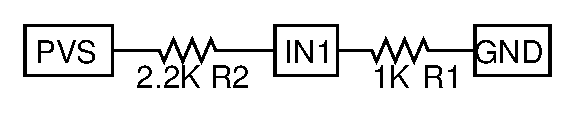
\includegraphics[height=0.8cm]{schematics/resistors}
\begin{itemize}
\item Set PVS to some voltage, read the actual value set from the message
field.
\item Click on IN1 to measure its voltage.
\item Repeat for different values of PVS. 
\item Repeat for other resistance values.
\end{itemize}

\subsection*{Observation}

The total voltage and the voltage across R1 are measured. The voltage
across R2 is $V_{PVS}-V_{R1}$. The current through R1, $I=V_{R1}/R1$.
The same amount of current flows through R2 and the voltage across
R2 can be calculated using $V_{R1}=IR1$.

\begin{tabular}{|c|c|c|c|c|}
\hline 
{\footnotesize{$V_{PVS}$}} & {\footnotesize{$V_{IN1}=V_{R1}$}} & {\footnotesize{$I=\frac{V_{IN1}}{1000}$A}} & {\footnotesize{$V_{R2}=V_{PVS}-V_{IN1}$}} & {\footnotesize{$V_{R2}=I\times2.2k$}}\tabularnewline
\hline 
\hline 
1 & .313 & .313 & .687 & .688\tabularnewline
\hline 
2 & .626 & .626 & 1.374 & 1.377\tabularnewline
\hline 
3 & .94 & .94 & 2.06 & 2.07\tabularnewline
\hline 
\end{tabular}

Expand this experiment by connecting three resistors in series and
connecting the junctions to IN1 and IN2. Another exercise is to connect
a $5.1k$ resistor from SEN to GND and measure the voltage at SEN.
Remember that SEN is internally connected to 5 volts through a $5.1k$
resistor.


\section{Calibrating Current Source\label{sec:Calibrating-Current-Source}}


\subsection*{Objective}

The actual output of constant current source may be different from
the specified 1 mA, due to the tolerance of the resistors used. It
can be measured by connecting an ammeter from CCS to GND, or by connecting
a known resistance to CCS and measuring the voltage across it. The
resistor should be in 2k to 4k range.


\subsection*{Procedure}

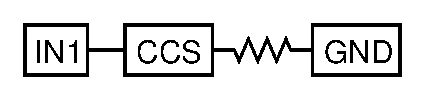
\includegraphics[height=0.8cm]{schematics/ccs-calib}
\begin{itemize}
\item Enable CCS 
\end{itemize}

\subsection*{Observation}

The measured values of the resistance is 3.876k and the voltage is
3.725 volts. The actual value of the constant current source is 3.725/3.876
= .961 mA. 

For better accuracy, the measured value should be used in experiments
using CCS.


\section{Resistances in series}


\subsection*{Objective}

Finding the effective resistance of a series combination of resistors,
$R=R1+R2+\cdots$, using a constant current source. A $560\Omega$
and a$1k\Omega$ resistors are used. 


\subsection*{Procedure}

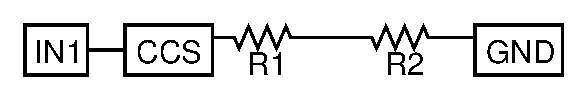
\includegraphics[height=0.8cm]{schematics/res-series}
\begin{itemize}
\item Connect R1, R2 alone and then both
\item Measure IN1 for each case
\end{itemize}

\subsection*{Observation}

\begin{tabular}{|c|c|}
\hline 
R($\Omega)$ & V(volts)\tabularnewline
\hline 
\hline 
560 & .558\tabularnewline
\hline 
1000 & 0.998\tabularnewline
\hline 
1000+560 & 1.556\tabularnewline
\hline 
\end{tabular}

Since the current is same, the total voltage drop gives the effective
resistance. It can be seen that it is the sum of the individual values,
within the measurement error. For more accurate results, use the value
of current measured as explained in section \ref{sec:Calibrating-Current-Source},
instead of 1mA.


\section{Resistances in parallel}


\subsection*{Objective}

Find the effective resistance of parallel combination of resistors,
given by $\frac{1}{R}=\frac{1}{R1}+\frac{1}{R2}+\cdots$


\subsection*{Procedure }

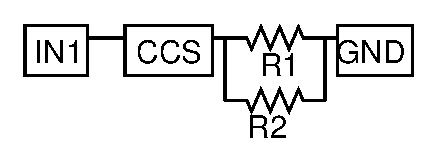
\includegraphics[height=1cm]{schematics/res-parallel}
\begin{itemize}
\item Connect 1$k\Omega$ resistor from CCS to Ground.
\item Repeat the same with two resistors connected in parallel.
\end{itemize}

\subsection*{Observation}

\begin{tabular}{|c|c|}
\hline 
$R_{connected}(\Omega)$ & $V_{measured}(V)$\tabularnewline
\hline 
\hline 
1000 & 1.008\tabularnewline
\hline 
1000$\parallel$1000 & 0.503\tabularnewline
\hline 
\end{tabular}

Since we know the current, we can calculate the resistance from the
measured voltage. As per the measured voltage the resistance of the
parallel combination is $\frac{0.503V}{0.001A}=503\Omega$.


\section{Measure resistance by comparison\label{sec:Measure-resistance-by}}


\subsection*{Objective}

Learn to apply Ohm's law to find the value of an unknown resistance
by comparing it with a known one. Voltage across a resistor is given
by $V=IR$ . If same amount of current is flowing through two different
resistors, the ratio of voltages will be the same as the ratio of
resistances, $I=\frac{V1}{R1}=\frac{V2}{R2}$.


\subsection*{Procedure }


\includegraphics[height=0.8cm]{schematics/res-compare}
\begin{itemize}
\item Connect the unknown resistor R from PVS to IN1.
\item Connect 1$k\Omega$ (R1) from IN1 to Ground.
\item Set PVS to 4 volts.
\item Measure voltage at IN1
\end{itemize}

\subsection*{Observation}

Voltage at IN1 = 1.254, implies voltage across the unknown resistor
is $4-1.254=2.746$

Current $I=\frac{1.254}{1000}=1.254mA$ . Unknown resistor value =
$\frac{2.746}{1.254mA}=2.19k\Omega$

What is the limitation of this method ? How do we choose the reference
resistor ? suppose the unknown value is in Mega Ohms, what will be
the voltage drop across a $1k\Omega$ reference resistor ? Our voltage
measurement is having a resolution of $\frac{1}{4095}$.

We will use this method later to measure the resistance of solutions,
using AC.


\section{Voltage of a lemon cell }


\subsection*{Objective}

Make a voltage source by inserting Zinc and Copper plates into a lemon.
Explore the current driving capability and internal resistance.


\subsection*{Procedure }


\subsection*{\protect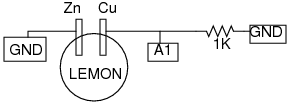
\includegraphics[height=1.3cm]{schematics/lemon-cell}}
\begin{itemize}
\item Click on A1 to measure voltage
\item Measure the voltage with and without the 1k resistor
\end{itemize}

\subsection*{Observation}

Voltage across the Copper and Zinc terminals is nearly .9 volts. Connecting
the resistor reduces it to 0.33 volts. When connected, current will
start flowing through the resistor. But why is the voltage going down
?

What is the internal resistance of the cell ?

Current is the flow of charges and it has to complete the path. That
means, current has to flow through the cell also. Depending on the
internal resistance of the cell, part of the voltage gets dropped
inside the cell itself. Does the same happen with a new dry-cell ?


\section{DC, AC and power line pickup}


\subsection*{Objective}

Introduce the concept of time dependent voltages, using a V(t) graph.
Compare the graph of DC and AC. Learn about the AC mains supply. Explore
the phenomenon of propagation of AC through free space.

\begin{figure}
\begin{centering}
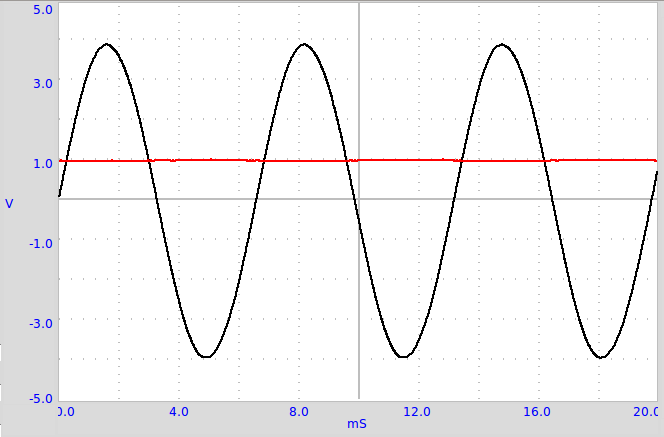
\includegraphics[width=5cm]{pics/ad-dc} 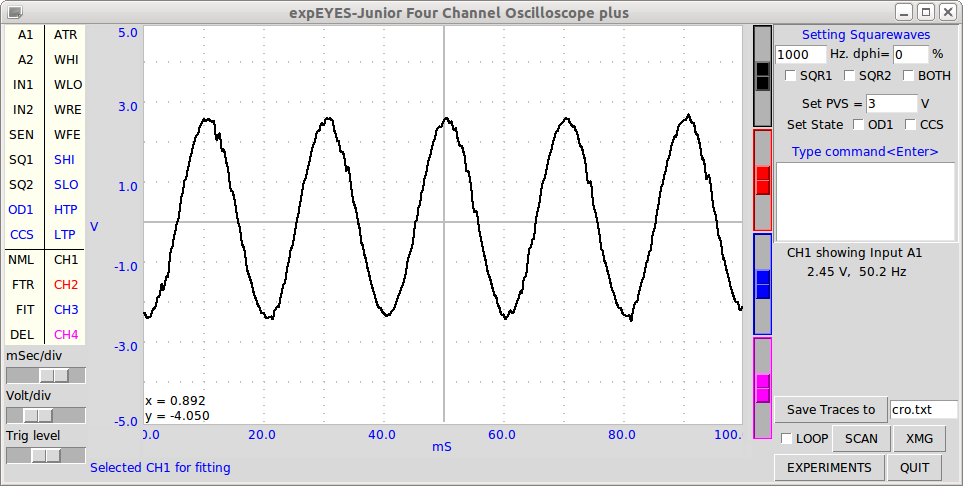
\includegraphics[width=6cm]{pics/pickup}
\par\end{centering}

\caption{Plotting Voltage Vs Time. (a) graph of DC and AC (b) AC mains pickup
\label{fig:Graph-of-DC}}
\end{figure}



\subsection*{Procedure }

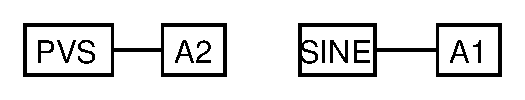
\includegraphics[height=0.7cm]{schematics/ac-dc} 
\begin{itemize}
\item Assign A1 to CH1 and A2 to CH2
\item Set PVS to 1 volt
\item Assign CH1 to FIT, to measure AC parameters.
\item Remove SINE and connect a long wire to A2
\end{itemize}
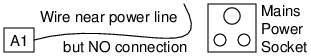
\includegraphics[height=1cm]{schematics/line-pickup}


\subsection*{Observation}

Figure \ref{fig:Graph-of-DC}(a) shows that the graph of DC is horizontal
line and for AC it changes direction and magnitude with time. The
voltage is changing with time. It goes to both negative and positive
around 150 cycles per second. This voltage waveform is generated by
using electronic circuits.

Enabling FIT option calculates the amplitude and frequency by fitting
the data with the equation $V=V_{0}\sin(2\pi ft+\theta)$ , where
$V_{0}$ is the amplitude and $f$ ~is the frequency. What is the
significance of $\theta$ in this equation ?

The power line pickup is shown in figure \ref{fig:Graph-of-DC}(b).
The frequency is obtained by fitting the data. Without making any
connection, how are we getting the AC voltage from the mains supply
?


\section{DC \& AC components of a voltage\label{sec:DC-&-AC}}


\subsection*{Objective}

Separating AC and DC components of a voltage waveform using a capacitor.

\begin{figure}
\begin{centering}
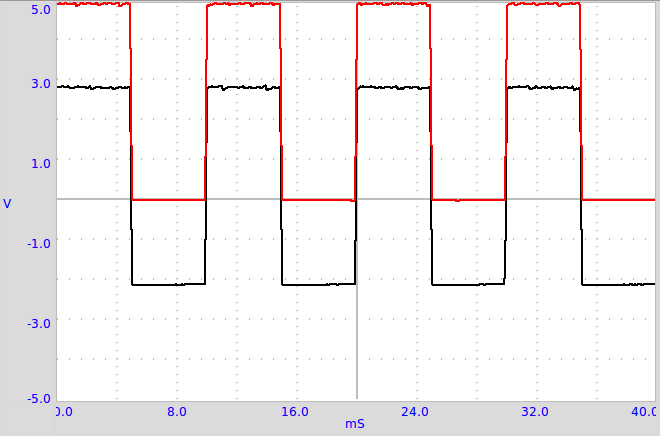
\includegraphics[width=6cm]{pics/acdc-sep-screen} 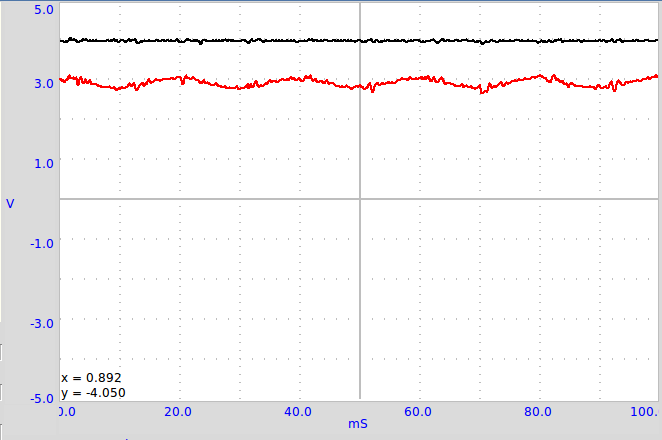
\includegraphics[width=5cm]{pics/body-resistance}
\par\end{centering}

\caption{(a) A 0 to 5V square wave, with DC component blocked (b) Resuming
electrical resistance of human body\label{fig:Square-wave}}
\end{figure}



\subsection*{Procedure }


\includegraphics[height=0.8cm]{schematics/acdc-separating}
\begin{itemize}
\item Set SQR1 to 500 Hz
\item Assign SQR1 to CH1 and A2 to CH2
\item Adjust the horizontal scale to see several cycles.
\end{itemize}

\subsection*{Observation}

The observed waveforms with and without the series capacitor are shown
in figure \ref{fig:Square-wave}. The voltage is swinging between
0 and 5 volts. After passing through the capacitor the voltage swings
from -2.5 volts to +2.5 volts.

What will you get if you subtract a 2.5 from the y-coordinate of every
point of the first graph? That is what the capacitor did. It did not
allow the DC part to pass through. This original square wave can be
considered as a 2.5V AC superimposed on a 2.5V DC.

You may need to connect a resistor from A2 to GND to see a waveform
swinging between -2.5 to +2.5 volts. Remove the resistor and observe
the result. 


\section{Resistance of human body}


\subsection*{Objective}

Get some idea about the resistance of the skin and how it varies.


\subsection*{Procedure}

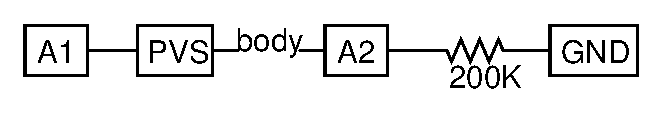
\includegraphics[height=0.8cm]{schematics/res-body}
\begin{itemize}
\item Assign A1 to CH1 and A2 to CH2
\item Join PVS and A2, through your body and measure voltage at CH2
\item Calculate your body's resistance, as given in section \ref{sec:Measure-resistance-by}
\item Repeat using SINE instead of PVS. Enable FIT to measure voltage.
\end{itemize}

\subsection*{Observation}

The observed waveform is shown in figure \ref{fig:Square-wave}(b).
Voltage at A2 is 3V, the variation is due to the 50Hz AC pickup. 


\section{Temperature dependent resistors }


\subsection*{Objective}

Show the dependence of resistance on temperature, using a thermistor,$1k\Omega@25^{0}C$,
with negative temperature coefficient. Introduce temperature sensor.


\subsection*{Procedure}

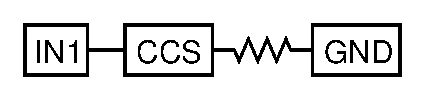
\includegraphics[height=0.8cm]{schematics/thermistor}
\begin{itemize}
\item Click on IN1 to measure the voltage
\item Repeat at different temperatures
\end{itemize}

\subsection*{Observation}

\begin{tabular}{|c|c|c|}
\hline 
Setup & V=IR & $R=\frac{V}{I}$\tabularnewline
\hline 
\hline 
In cold water & 1.2 & 1200\tabularnewline
\hline 
Room Temperature & 0.935 & 935\tabularnewline
\hline 
\end{tabular}


\section{Light dependent resistors}


\subsection*{Objective}

Learn about LDR. Measure intensity of light and its variation with
distance from the source. Use the comparison method to find out the
resistance.


\subsection*{Procedure }


\includegraphics[height=0.8cm]{schematics/ldr}
\begin{itemize}
\item Set PVS to 4V and note down the value set
\item Click on IN1 to measure it, Assign IN1 to CH1.
\item Calculate the LDR's resistance, as explained in\ref{sec:Measure-resistance-by}
\item Repeat by changing intensity of light falling on LDR
\item Connect an LED from SQR1 to GND. Set SQR1 to 10 Hz
\item Show the LED above LDR and watch waveform at IN1
\end{itemize}

\subsection*{Observation}

The resistance vary from 1k$\Omega$ to around 100 k$\Omega$ depending
on the intensity of light falling on it. The voltage is proportional
to the resistance. The resistance decreases with intensity of light.
If you use a point source of light, the resistance should increase
as the square of the distance.

Illuminate the LDR using a fluorescent tube and watch the waveform
at CH1. The frequency of the ripple is related to the mains frequency.


\section{Conductivity of water, using DC \& AC}


\subsection*{Objective}

Measure the resistance of ionic solutions, using both DC and AC voltages.
We have used normal tap water.


\subsection*{Procedure}
\begin{itemize}
\item R1 should be comparable to R, start with 10k.
\item Assign A1 to CH1 and A2 to CH2, enable FIT on both
\item Calculate the resistance as explained in section \ref{sec:Measure-resistance-by}
\item Repeat using a DC voltage, PVS instead of SINE
\end{itemize}

\subsection*{Observation}

\begin{figure}
\begin{centering}
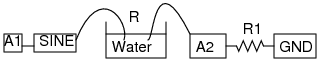
\includegraphics[width=5cm]{schematics/res-water} 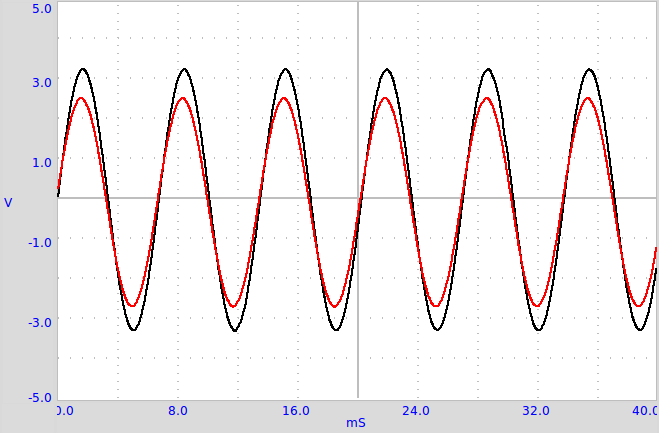
\includegraphics[width=5cm]{pics/water-conduct}
\par\end{centering}

\caption{Conductivity of water. (b)Total voltage applied and the voltage across
the 10k resistor.\label{fig:Conductivity-of-water.}}
\end{figure}


\begin{tabular}{|c|c|c|c|c|c|}
\hline 
 & $V_{total}$ & $V_{10k\Omega}$ & $V_{liq}$ & $I=\frac{V_{10k\Omega}}{1000}$ & $R_{liq}=\frac{V_{liq}}{I}$\tabularnewline
\hline 
\hline 
SINE & 3.25 & 2.6 & 0.65 & .26 mA & 2.5 k$\Omega$\tabularnewline
\hline 
PVS & 4 & 2.3 & 1.7 & .23 mA &  7.4 k$\Omega$\tabularnewline
\hline 
\end{tabular}

Observed values are shown in the table. The DC and AC resistances
seems to be very different. With DC, the resistance of the liquid
changes with time, due to electrolysis and bubble formation. The resistance
does not depend much on the distance between the electrodes, the area
of the electrode is having some effect. The resistance depends on
the ion concentration and presence of impurities in the water used.

Try changing the distance between electrodes. Try adding some common
salt and repeat the measurements. Why is the behavior different for
AC and DC ? What are the charge carriers responsible for the flow
of electricity through solutions ? Is there any chemical reaction
taking place ?


\section{Measuring Capacitance}


\subsection*{Objective}

expEYES Junior has an internal programmable current source, that can
be enabled on IN1. Connect a capacitance C and switch on current (5.5
$\mu A$) for a fixed time interval. The accumulated charge $Q=It=CV$
. By measuring $V$ , the value of C is calculated. For better results
the stray capacitance need to be subtracted. Measure C without connecting
anything to IN1, and subtract that value from the C measured with
capacitor. This method can be used for values upto 10000 pF.%
\footnote{Beyond that you need to use the Python function that can specify the
charging current, duration of charging etc.%
} Touching the capacitor during the measurement will corrupt the result. 


\subsection*{Procedure }


\includegraphics[height=0.8cm]{schematics/measure-cap}
\begin{itemize}
\item Measure C without anything connected, to get the stray capacitance.
\item connect the capacitor from IN1 to ground. 
\item Click on the Button\menuitem{Measure C on IN1}
\item Repeat with different capacitors
\end{itemize}

\subsection*{Observation}

The empty socket measures 34 pF. Several capacitors were measured.

\begin{tabular}{|c|c|}
\hline 
 Value & Measured value (pF) - 34pF\tabularnewline
\hline 
\hline 
10 & 11\tabularnewline
\hline 
20 & 19\tabularnewline
\hline 
680 & 664\tabularnewline
\hline 
180 & 176\tabularnewline
\hline 
3000 & 2900\tabularnewline
\hline 
\end{tabular}


\section{Measuring Dielectric Constant}


\subsection*{Objective}

Measure the dielectric constant of materials like glass, paper, polyester
etc., by making a capacitor. Capacitance $C=\epsilon_{0}k\frac{A}{d}$,
where $\epsilon_{0}$ is the permittivity of free space, $k$ the
dielectric constant , $A$ the overlapping area of plates and $d$
the separation between them. We have used a 13 cm x 10.6 cm piece
of window glass having 4 mm thickness to make a capacitor by pasting
metal foil on both sides.


\subsection*{Procedure }
\begin{itemize}
\item connect the capacitor from IN1 to ground. 
\item Click on the Button \menuitem{Measure C on IN1}
\item Repeat without connecting anything to IN1
\end{itemize}

\subsection*{Observation}

The measured capacitance is 225 pF. The stray capacitance is measured
after removing the wire from IN1 and it is 30pF, means C = 195pF.
$k=\frac{Cd}{\epsilon_{0}A}=\frac{195e-12\times0.004}{8.854e-12\times.13\times.106}=6.37$.
Touching the capacitor during the measurement gives wrong results. 

Using two parallel plates, the dielectric constant of liquids also
can be measured.


\section{AC Phase shift in RC circuits\label{sec:Capacitor-in-AC}}


\subsection*{Objective}

Explore the effect of a series capacitor in AC circuits, under steady
state conditions. Impedance of a Capacitor $X_{c}=\frac{1}{2\pi fC}$
, where $f$ is the frequency in Hertz and $C$ is the capacitance
in Farads. 


\subsection*{Procedure}

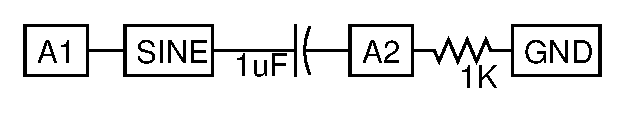
\includegraphics[height=0.8cm]{schematics/rc-acphase}
\begin{itemize}
\item Assign A1 to CH1 and A2 to CH2
\item Adjust the horizontal scale to view more than 4 cycles.
\item Right click on CH1 to calculate the phase shift.
\end{itemize}
For a detailed study select \textit{\menuitem{Study of AC Circuits}}
from \textit{\menuitem{EXPERIMENTS}.}


\subsection*{Observation}

The voltage waveform before and after the capacitor are shown in figure
\ref{fig:AC-Phase-in-RC}(a),and the calculations are shown in the
table.

\begin{tabular}{|c|c|c|c|c|}
\hline 
C(uF) & R($\Omega$) & Freq (Hz) & $\bigtriangleup\Phi$ & $\arctan\left(\frac{X_{c}}{X_{R}}\right)$\tabularnewline
\hline 
\hline 
1 & 1000 & 147.3 & 47.7 & 47.2\tabularnewline
\hline 
\end{tabular}

where $X_{c}=\frac{1}{2\pi fC}$ is the impedance of the capacitor,
Frequency is 147.3 Hz. $X_{R}$ is the resistance.

Current through a capacitor leads the voltage across it by $90^{0}$.
Why ?

Why does the phase of the voltage advance? Assume we have connected
the AC to plate A and at an instant $t=t_{0}$ the input voltage is
at zero volts. We can see that the slope of the curve is maximum there,
i.e. the rate of change of voltage is maximum. The capacitor gets
charged very fast at this point. The plate B also gathers the same
charge as plate A , that is how a capacitor works. The current to
plate B is flowing from ground through the resistor and we are measuring
the IR drop across the resistor, it will be already positive when
plate A is at zero. This results in the phase advance.
\begin{figure}
\begin{centering}
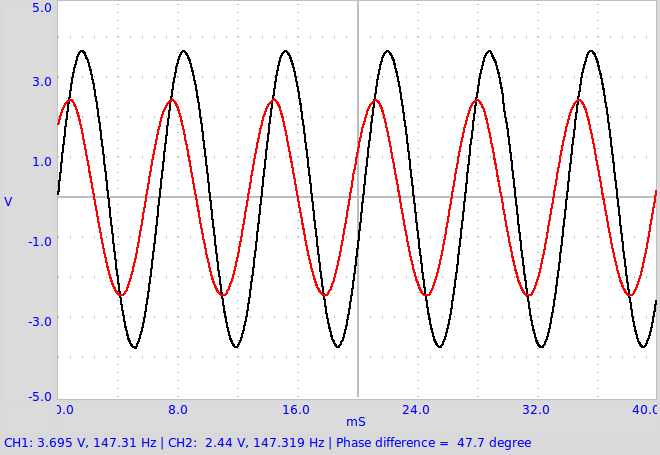
\includegraphics[width=5cm]{pics/rc-phaseshift} 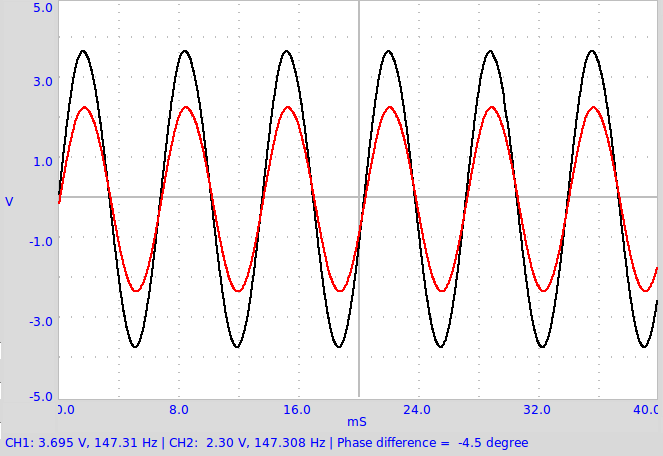
\includegraphics[width=5cm]{pics/rl-phaseshift}
\par\end{centering}

\caption{Phase shift of AC in an (a) RC circuit (b) RL circuit \label{fig:AC-Phase-in-RC}}
\end{figure}



\section{AC phase shift in RL circuits\label{sec:Inductor-in-AC}}


\subsection*{Objective}

Measure the AC voltage phase shift in an RL circuit. Impedance of
an Inductor $X_{L}=2\pi fL$ , where $f$ is the frequency in Hertz
and L is the inductance in Henry. In an LC circuit, the phase lag
across the inductor is given by the equation $\triangle\Phi=\arctan\left(\frac{X_{L}}{X_{R}}\right)$,
where R is the resistance in Ohms.


\subsection*{Procedure}


\includegraphics[height=0.8cm]{schematics/rl-acphase}
\begin{itemize}
\item Assign A1 to CH1 and A2 to CH2
\item Adjust the horizontal scale to view more than 4 cycles.
\item Right Click on A1 to view voltage, frequency and phase difference.
\end{itemize}

\subsection*{Observation}

The measured phase shifts are shown below. Waveforms for the 125 mH
inductor is shown in figure \ref{fig:AC-Phase-in-RC}(b). The resistance
of the inductor also should be included while calculating the phase
shift.%
\footnote{http://www.play-hookey.com/ac\_theory/ac\_inductors.html%
}.

\begin{tabular}{|c|c|c|c|}
\hline 
L(mH) & $R=R_{coil}+R_{ext}$($\Omega$) & $\bigtriangleup\Phi=\arctan\left(\frac{X_{L}}{X_{R}}\right)$ & $\bigtriangleup\Phi_{measured}$\tabularnewline
\hline 
\hline 
125 & 565 + 560 & 3.71 & -3.8\tabularnewline
\hline 
\end{tabular}

Insert an iron or ferrite core to the coil and observe the effect
of ferromagnetic materials. Self Inductance of a solenoid is given
by $L=\frac{\mu N^{2}A}{l}$ , where N is the number of turns, A is
the cross sectional area, $\mu$ is the permeability of the surrounding
media and $l$ is the length.


\section{Transient Response of RC circuits\label{sec:Capacitor-charging-&}}


\subsection*{Objective}

Plot the voltage across a capacitor, when it is charged by applying
a voltage step through a resistor. Calculate the value of the capacitance
from the graph.


\subsection*{Procedure}


\includegraphics[height=0.8cm]{schematics/RCcircuit} 
\begin{itemize}
\item From \textit{\menuitem{EXPERIMENTS}} , select \textit{\menuitem{RC Circuit}} 
\item Click on \textit{0->5V STEP} and \textit{5->0V step} Buttons to plot
the graphs
\item Adjust the horizontal scale, if required, and repeat.
\item Calculate RC time constant.
\item Use CCS instead of OD1 to charge capacitor with constant current.
\end{itemize}

\subsection*{Observation}

\begin{figure}
\begin{centering}
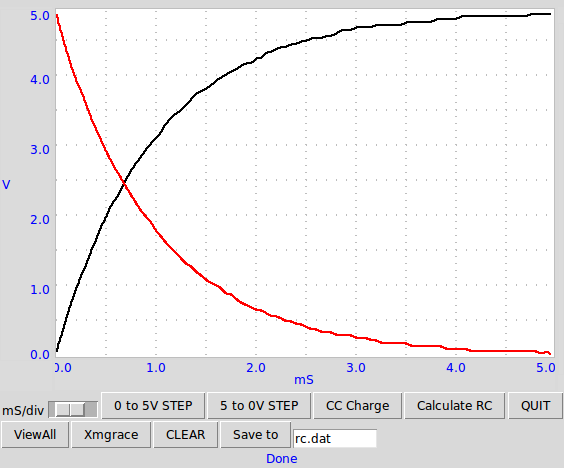
\includegraphics[width=5cm]{pics/RC-curves} 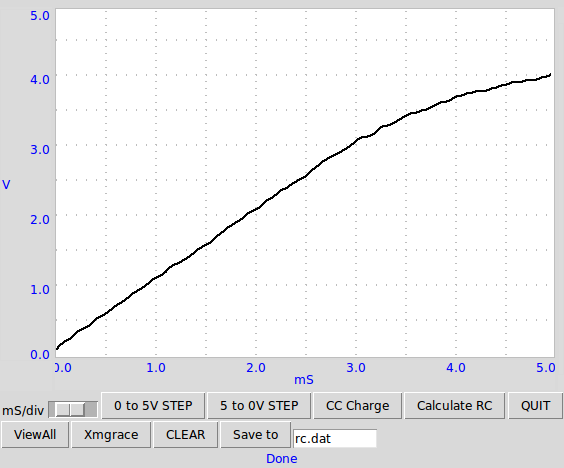
\includegraphics[width=5cm]{pics/cap-linear}
\par\end{centering}

\caption{(a)Transient response of RC circuit. (b) Charging of capacitor with
constant current. \label{fig:Transient-RC}}
\end{figure}


Applying a 0 to 5V step makes the voltage across the capacitor to
rise exponentially as shown in the figure\ref{fig:Transient-RC}(a).
By fitting the discharge curve with $V(t)=V_{0}e^{-\frac{t}{RC}}$
,we can extract the RC time constant and find the values of capacitance
from it. 

The voltage across a capacitor is exponential only when it is charged
trough a linear element, a resistor for example. When charged from
a constant current source, the voltage shows linear increase, as shown
in figure \ref{fig:Transient-RC}(b), because $Q=It=CV$ , and voltage
increases linearly with time as $V=\left(\frac{I}{C}\right)t$ .


\section{Transient Response of RL circuits}


\subsection*{Objective}

Explore the nature of current and voltage when a voltage step is applied
to resistor and inductor in series. By measuring the voltage across
the inductor as a function of time, we can calculate its inductance.

In an RL circuit $V=IR+L\frac{dI}{dt}$ and solving this will give
$I=I_{0}e^{-\frac{R}{L}t}$. The coefficient of the exponential term
R/L can be extracted from the graph of voltage across the inductor.
The resistance of the inductor coil should be included in the calculations,
$R=R_{ext}+R_{L}$. %
\footnote{http://nptel.iitm.ac.in/courses/Webcourse-contents/IIT-KANPUR/esc102/node14.html%
}


\subsection*{Procedure}


\includegraphics[height=0.8cm]{schematics/RLcircuit}
\begin{itemize}
\item Inductor is the 3000 Turn coil
\item From \textit{\menuitem{EXPERIMENTS}} select \textit{\menuitem{RL Circuit}}
\item Click on \textit{0->5V STEP} and \textit{5->0V step} Buttons to plot
the graphs
\item Adjust the horizontal scale, if required, and repeat.
\item Calculate the value of inductance
\item Insert an iron core into the inductor and repeat
\end{itemize}

\subsection*{Observation}

\begin{figure}
\begin{centering}
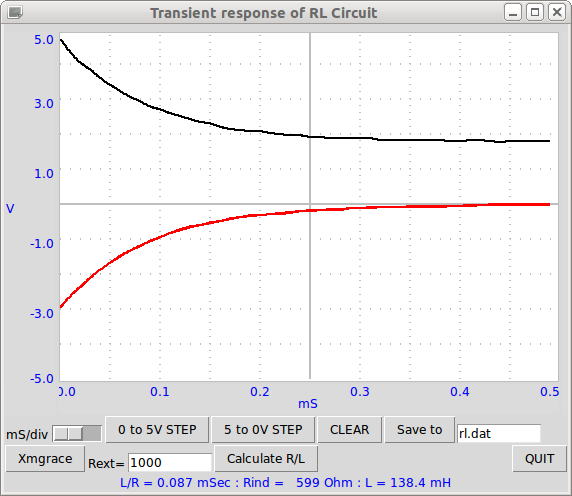
\includegraphics[width=5cm]{pics/RL-curves}
\par\end{centering}

\caption{Transient response of RL circuit\label{fig:Transient-RL}}
\end{figure}


The transient response of the inductor is shown in figure \ref{fig:Transient-RC}.
The exponential curve is fitted to extract the L/R value. The resistance
of the coil is measured by comparing it with the known external resistance
under DC conditions. IN1 is connected to OD1 for a more accurate measurement
of the coil resistance.

The applied voltages are above zero, but the graph went to negative
voltages. Why ?

What was the current before doing the 5->0 step ? What is back EMF
?

Repeat with two coils in series, by (a) placing them far away (b)
placing one over the other and (c) after changing the orientation.
The effect of mutual inductance can be seen.


\section{Transient response of LCR circuits\label{sec:Step-Response-ofRLC}}


\subsection*{Objective}

Explore the oscillatory nature of L and C in series. Resonant frequency
of series LC circuit is given by $\omega_{0}=\frac{1}{2\pi\sqrt{LC}}$.
The damping factor is $\frac{R}{2}\sqrt{\frac{C}{L}}$, and it is
equal to 1 for critical damping.%
\footnote{http://en.wikiversity.org/wiki/RLC\_circuit%
} Depending upon the value of C/L and R, the response could be under-damped,
critically-damped or over-damped. 

\begin{figure}
\begin{centering}
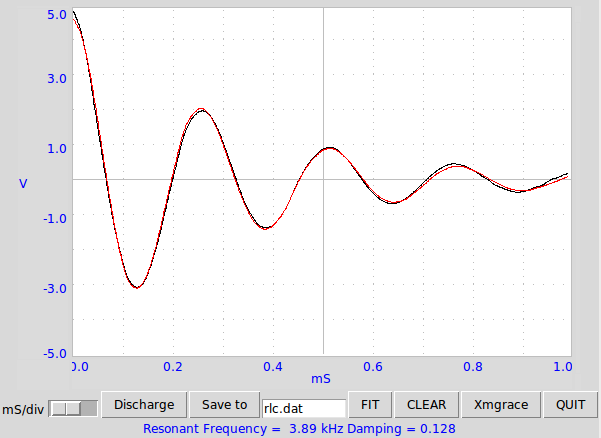
\includegraphics[width=5cm]{pics/RLC-curves} 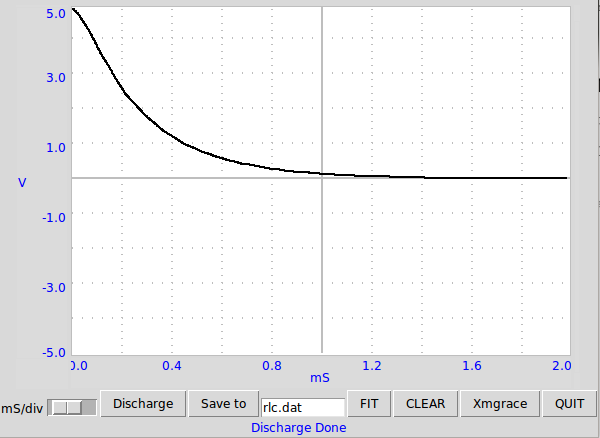
\includegraphics[width=5cm]{pics/RLC-curve-damped}
\par\end{centering}

\caption{Transient response of LCR circuit,(a)Under-damped (b)Over-damped.\label{fig:LCR Transient-response}}
\end{figure}



\subsection*{Procedure }


\includegraphics[height=0.8cm]{schematics/LCRcircuit} 
\includegraphics[height=0.7cm]{schematics/LCRRcircuit}
\begin{itemize}
\item From \textit{\menuitem{EXPERIMENTS}} select\textit{ \menuitem{RLC Discharge}} 
\item Click on 5->0V STEP. Adjust x-axis and repeat if required.
\item FIT the graph to find the resonant frequency \& Damping.
\item Repeat the experiment with different values of L, C and R
\item Repeat with a resistor in series.
\end{itemize}

\subsection*{Observation}

We have used the 3000 turn coil and a 0.1uF capacitor, added a 2.2k
series resistor in the second case. The voltage across the capacitor
after a 5 to 0V step is shown in figure \ref{fig:LCR Transient-response}
.The measured resonant frequency tallies with $f=\frac{1}{2\pi}\sqrt{\frac{1}{LC}}$
, within the component tolerance values.


\section{RC Integration \& Differentiation }


\subsection*{Objective}

RC circuits can integrate or differentiate a voltage waveform with
respect to time. A square wave is integrated to get a triangular wave
and differentiated to get spikes at the transitions.


\subsection*{Procedure}


\includegraphics[height=0.8cm]{schematics/rc-integ} 
\begin{itemize}
\item Set SQR2 to 1000Hz
\item Assign SQR2 to CH1 and A1 to CH2
\item Adjust the horizontal scale to view more than 4 cycles.
\item Set SQR2 to 1kHz (T = 1mS) and other values and view the waveforms.
\item Repeat the same for RC differentiator, at 100Hz.
\end{itemize}

\includegraphics[height=0.8cm]{schematics/rc-diff}


\subsection*{Observation}

\begin{figure}
\begin{centering}
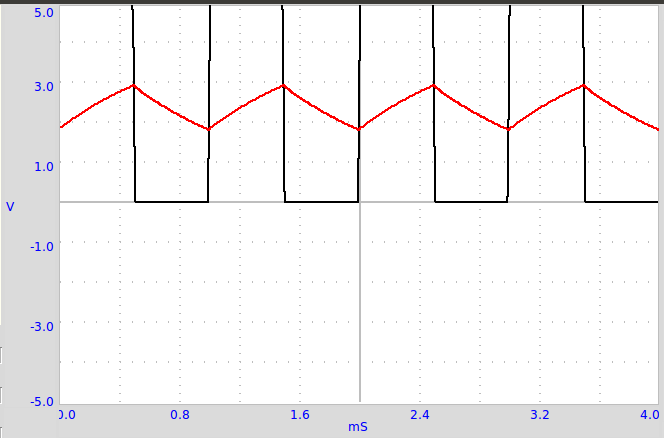
\includegraphics[width=5cm]{pics/rc-integ1khz}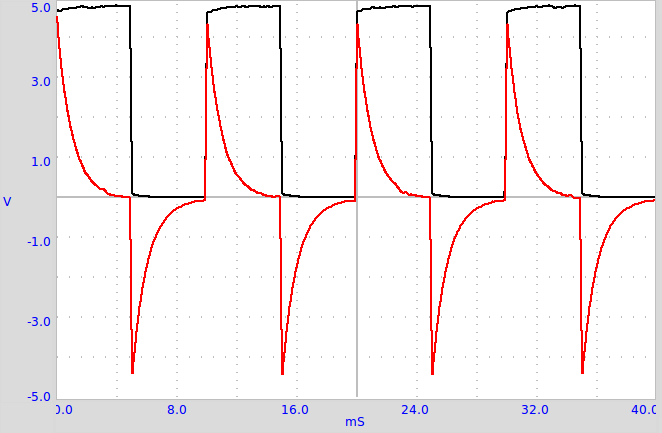
\includegraphics[width=5cm]{pics/rc-diff100Hz}
\par\end{centering}

\caption{(a)1kHz Squarewave after RC Integrator (b) 100Hz after RC Differentiator\label{fig:RC-int-diff}}
\end{figure}


Integration observed at 1kHz and differentiation at 100Hz are shown
in figure \ref{fig:RC-int-diff}, using an RC value of 1 milliseconds.
When the time period becomes comparable with the RC value, the output
waveform is triangular. The differentiation can only be shown at lower
frequency since capturing the narrow spike requires a fast oscilloscope.


\section{Fourier Analysis\label{sec:Fourier-Transform-**}}


\subsection*{Objective}

Learn about Fourier Transform of a signal. Time and Frequency domain
representations.


\subsection*{Procedure}

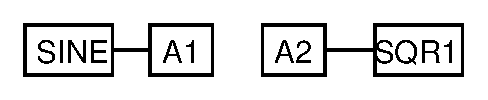
\includegraphics[height=0.8cm]{schematics/ftran}
\begin{itemize}
\item Set SQR1 to 150Hz
\item Assign A1 to CH1 and SQR1 to CH2
\item Assign CH1 \& CH2 to FT to view the Fourier transform
\end{itemize}

\subsection*{Observation}

\begin{figure}
\begin{centering}
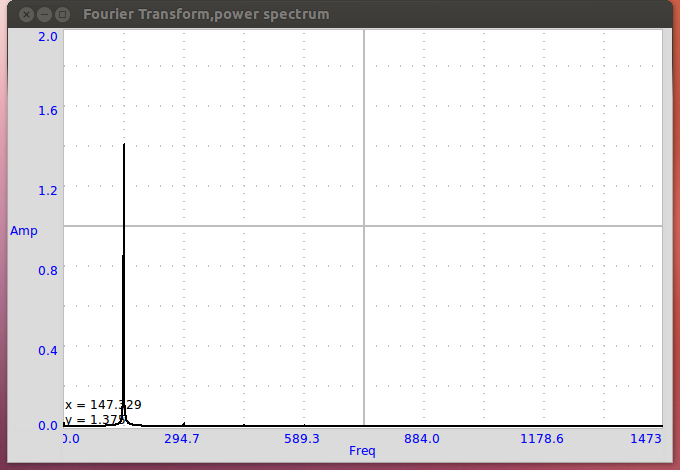
\includegraphics[width=5cm]{pics/fft-sine147Hz} 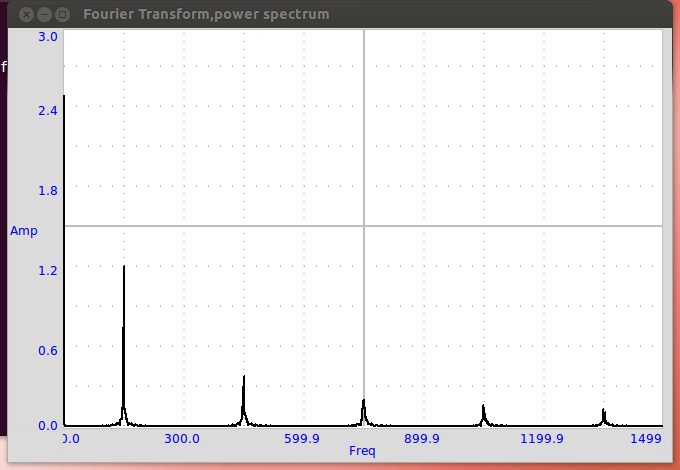
\includegraphics[width=5cm]{pics/fft-sqr150Hz}
\par\end{centering}

\caption{Frequency spectrum of (a)Sine wave. (b) Squarewave\label{fig:Frequency-spectrum-of}}
\end{figure}


In the Fourier transform plot, frequency is on the x-axis and the
y-axis shows the relative strength of each frequency components of
the signal. This is called the frequency domain representation%
\footnote{http://en.wikipedia.org/wiki/Fourier\_transform%
}. For the sine wave there is only one dominant peak, the smaller ones
are a measure of distortion of the sine wave. 

A square wave function can be represented as $f(\theta)=sin(\theta)+\frac{sin(3\theta)}{3}+\frac{sin(5\theta)}{5}+\cdots$.
In the Fourier transform of a square wave of frequency $f$ , there
will be a $3f$ component (having an amplitude of one third of $f$
), $5f$ component (amplitude one fifth) etc. as shown in the figure
\ref{fig:Frequency-spectrum-of}(b). Note the peak at 0 Hz, due to
the DC component.


\chapter{Electricity \& Magnetism}

Electromagnetic induction is demonstrated by dropping a magnet in
to a coil. Working of transformer is demonstrated using two coils.
A simple AC generator, capable of generating multi-phase output, is
made using a rotating magnet.


\section{Electromagnetic induction}


\subsection*{Objective}

Explore the voltage induced across a coil by a changing magnetic field,
by dropping a small cylindrical magnet into a coil. Use a tube to
guide the magnet through the coil.


\subsection*{Procedure}

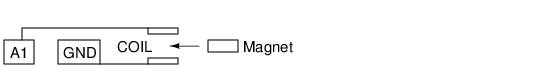
\includegraphics[height=1cm]{schematics/induction}
\begin{itemize}
\item From \menuitem{EXPERIMENTS}open \menuitem{EM Induction}
\item Click on Start Scanning. A horizontal trace should appear
\item Drop the magnet through the coil, until a trace is caught.
\item Repeat the process by changing the parameters like magnet strength,
speed etc.
\end{itemize}

\subsection*{Observation }

\begin{figure}
\begin{centering}
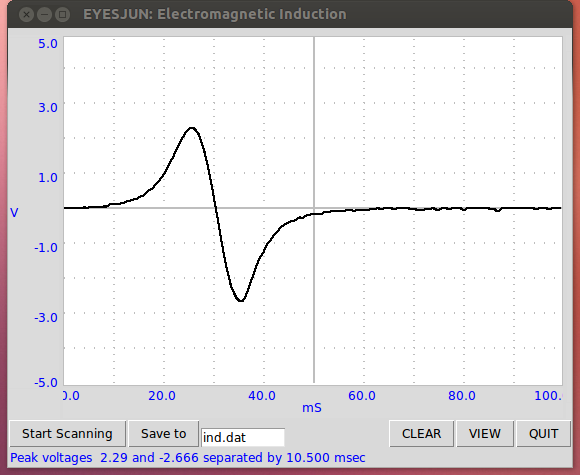
\includegraphics[width=5cm]{pics/induction-screen} 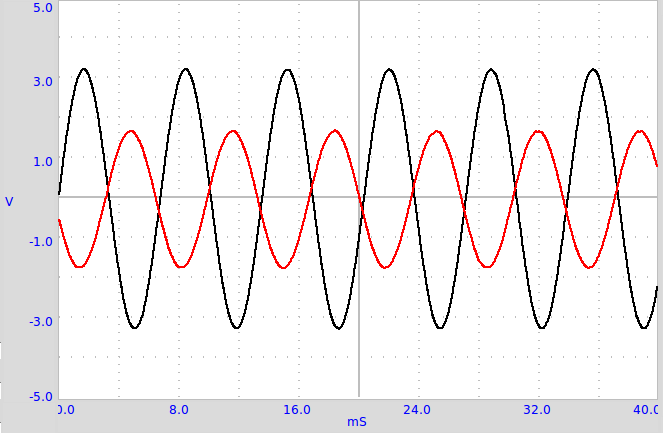
\includegraphics[width=5cm]{pics/transformer-screen}
\par\end{centering}

\caption{(a)Voltage induced on a coil by a moving magnet.(b)Mutual Induction
between two coils, the applied and induced voltages are shown \label{fig:Voltage-induced-on}}
\end{figure}


The result is shown in figure \ref{fig:Voltage-induced-on}(a). The
amplitude increases with the speed of the magnet. From the graph,
we can find the time taken by the magnet to travel through the coil.

The second peak is bigger than the first peak. Why ? Where will be
the magnet at the zero crossing of the induced voltage? Drop the magnet
from different heights and plot the voltage vs square root of the
height.


\section{Mutual induction, transformer}


\subsection*{Objective}

Demonstrate mutual induction using two coils. One coil is powered
by the SINE output. The axes of the coils are aligned and a ferrite
core is inserted.


\subsection*{Procedure}

\begin{flushleft}

\includegraphics[height=1cm]{schematics/tran}
\par\end{flushleft}
\begin{itemize}
\item Assign A1 to CH1 and A2 to CH2
\end{itemize}

\subsection*{Observation}

The applied waveform and the induced waveform are shown in figure
\ref{fig:Voltage-induced-on}(2). A changing magnetic filed is causing
the induced voltage. In the previous two experiments, the changing
magnetic field was created by the movement of permanent magnets. In
the present case the changing magnetic field is created by a time
varying current.

The output should have been in phase with the input as per the theory.%
\footnote{http://sound.westhost.com/xfmr.htm%
}However, this is not happening if the coupling is not enough. With
more ferrite material, the phase shift is as expected from the theory.
Try doing this experiment using a squarewave of 100 Hz, 1000 Hz etc.
Connect a 1k$\Omega$ resistor across secondary coil to reduce ringing.


\section{A simple AC generator\label{sec:A-simple-AC}}


\subsection*{Objective}

Measure the frequency and amplitude of the voltage induced across
a solenoid coil by a rotating magnet. Gain some understanding about
the AC generators by looking at the output and the drawbacks of the
setup. Use the 10 mm x 10 mm magnet and the 3000T coils that comes
with the kit.

\begin{figure}
\begin{centering}
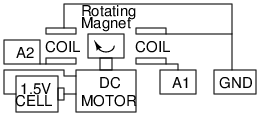
\includegraphics[width=4cm]{schematics/ac-generator} 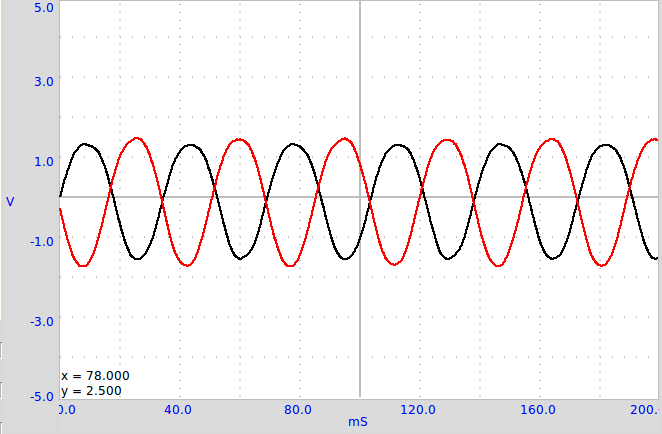
\includegraphics[width=4cm]{pics/ac-gen-screen}
\par\end{centering}

\caption{Wiring schematic and voltage output of the AC generator, with coils
placed on opposite sides of the rotating magnet.\label{fig:AC generator output}.}
\end{figure}



\subsection*{Procedure}
\begin{itemize}
\item Mount the magnet horizontally and power the DC motor from a 1.5 volts
cell
\item Hold the coil perpendicular to the axis of rotation of the motor,
close to the magnet. Be careful not to touch it.
\item Assign A1 to CH1 \& A2 to CH2
\item Assign CH1 and CH2 to FIT
\end{itemize}

\subsection*{Observation}

The voltage output is shown in figure \ref{fig:AC generator output}.
The phase difference between the two voltages depends on the angle
between the axes of the two coils.

Bring a shorted coil near the magnet to observe the change in frequency.
The shorted coil is drawing energy from the generator and the speed
get reduced. The magnetic field in this generator is very weak. The
resistance of the coil is very high and trying to draw any current
from it will drop most of the voltage across the coil itself. 


\chapter{Electronics}

The non-linear elements like diodes and transistors are studied by
drawing their characteristic curves and making simple circuits to
demonstrate their functioning. Photo-transistor is used for transparency
measurements, optical signal transmission and for timing mechanical
movements. Amplitude and Frequency modulation are explored. A bread
board is required to carry out some of the experiments described in
this section.


\section{Half wave rectifier, PN junction}


\subsection*{Objective}

Learn the working of a PN junction diode. Making DC from a sinusoidal
AC. Filtering to reduce the AC component.

\begin{figure}
\begin{centering}
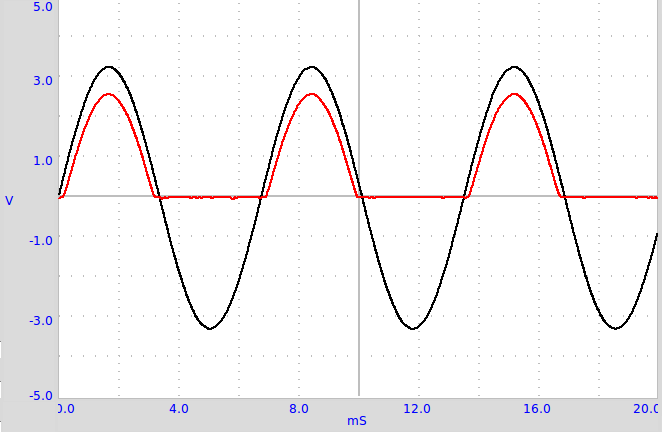
\includegraphics[width=5cm]{pics/half-wave-screen} \includegraphics[width=5cm]{pics/half-wave-filter-screen}
\par\end{centering}

\caption{(a) Half wave rectifier input and output.(b) With capacitor filter.\label{fig:Diode-rectifier} }
\end{figure}



\subsection*{Procedure }

\includegraphics[height=0.8cm]{schematics/half-wave}
\begin{itemize}
\item Assign A1 to CH1 and A2 to CH2
\item Add different values of filter capacitors from A2 to ground 
\end{itemize}

\subsection*{Observation}

The negative half is removed by the diode as shown in figure \ref{fig:Diode-rectifier}(a).
Also notice that the voltage in the positive half is reduced by around
0.7 volts, the voltage drop across a silicon diode. A load resistor
is required for the proper operation of the circuit, it could be more
than 1k$\Omega$ but do NOT use very low values since our AC source
can drive only up to 5 mA current.

The effect of a capacitor is shown in figure \ref{fig:Diode-rectifier}(b).
We can see that the capacitor charges up and then during the missing
cycle it maintains the voltage. The remaining AC component is called
the ripple in the DC.

Can we use very large capacitance to reduce the ripple ?

During what part of the cycle does current flow through the diode
?

Amount of peak current is decided by what ?


\section{180$^{\circ}$out of phase sine waves}


\subsection*{Objective}

To demonstrate the working of a full-wave rectifier using two diodes,
we need two AC waveforms, differing by 180 degree in phase. We do
this by inverting the output of SINE using an inverting amplifier.
The gain is made near unity by feeding the amplifier input through
a 51k$\Omega$ series resistor.

\begin{figure}
\begin{centering}
\includegraphics[width=5cm]{pics/ac-invert} \includegraphics[width=5cm]{pics/full-wave}
\par\end{centering}

\caption{(a)Inverting Amplifier making 180$^{\circ}$out of phase sine wave.(b)Fullwave
rectifier, two inputs and the output.\label{fig:Inverting-Amplifier-making}}
\end{figure}



\subsection*{Procedure }

\includegraphics[height=0.8cm]{schematics/ac-invert}
\begin{itemize}
\item Assign A1 to CH1 and A2 to CH2
\item Right-click on CH1 to measure phase difference
\end{itemize}

\subsection*{Observation}

The result is shown in the figure \ref{fig:Inverting-Amplifier-making}.
The amplitudes are not exactly equal. The gain is given by $G=\frac{51000}{51000+1000}$. 


\section{Fullwave rectifier}


\subsection*{Objective}

Make a full wave rectifier, using two diodes. Two AC waveforms, differing
by 180 degree in phase as required, are made as described in the previous
section. The rectified output is connected to the third channel. 


\subsection*{Procedure }

\includegraphics[height=1cm]{schematics/full-wave}
\begin{itemize}
\item Assign A1 to CH1, A2 to CH2 and IN1 to CH3
\item Add Capacitor from IN1 to ground , for filtering.
\end{itemize}

\subsection*{Observation}

The result is shown in the figure \ref{fig:Inverting-Amplifier-making}.
Adding capacitors to reduce the ripple is left as an exercise to the
user. This experiment is only to demonstrate the working of a full
wave rectifier, it cannot provide more than few milli amperes of current. 

Why full-wave rectifier is superior to half-wave rectifier ?


\section{Diode I-V characteristic}


\subsection*{Objective}

Draw the I-V Characteristic of diode and compare the result with the
theory. The IV characteristic of an ideal PN junction diode is given
by equation $I=I_{0}\left(e^{\frac{qV}{kT}}-1\right)$, where $I_{0}$
is the reverse saturation current, $q$ the charge of electron, $k$
the Boltzmann constant, $T$ the temperature in Kelvin. For a practical,
non-ideal, diode, the equation is $I=I_{0}\left(e^{\frac{qV}{nkT}}-1\right)$,
where $n$ is the ideality factor, that is $1$ for an ideal diode.
For practical diodes it varies from 1 to 2. We have used a IN4148
silicon diode.


\subsection*{Procedure}

\begin{flushleft}
\includegraphics[width=3cm]{schematics/diode-iv} 
\par\end{flushleft}
\begin{itemize}
\item From \menuitem{EXPERIMENTS} select \menuitem{Diode IV} .
\item Click on START to draw the characteristic curve.
\item Click on FIT to calculate the Diode Ideality factor.
\item Plot the IV of LEDs
\end{itemize}

\subsection*{Observation}

\begin{figure}
\begin{centering}
\includegraphics[width=5cm]{pics/diode-iv-screen} \includegraphics[width=5cm]{pics/led-iv-screen}
\par\end{centering}

\caption{I-V characteristic of (a) Silicon diode (b) several LEDs\label{fig:I-V-characteristic-of}}


\end{figure}


The curves obtained are shown in figure \ref{fig:I-V-characteristic-of}(a).
The value of n for 1N4148 is around 2. We have calculated the value
of $n$ by fitting the experimental data with the equation%
\footnote{If the FIT is not successful, transfer data to \textit{xmGrace} and
use the option Data->Transformations->Nonlinear curve fitting with
equation y=a0{*}exp(a1{*}x). %
}. Figure \ref{fig:I-V-characteristic-of}(b) shows the IV curves of
few LEDs, of different wavelengths. 

The voltage at which LED starts emitting light depends on its wavelength
and Planck's constant. Energy of a photon is given by $E=h\nu=hc/\lambda$
. This energy is equal to the energy of an electron that overcomes
the junction barrier and is given by $E=eV_{0}$. So Planck's constant
$h=eV_{0}\lambda/c$ , where $\lambda$ is the wavelength of light
from the LED, $e$ the charge of electron and $c$ the velocity of
light. 

Repeat the experiment by heating the diode to different temperatures.


\section{Transistor CE characteristic\label{sec:Transistor-CE-Characteristic}}


\subsection*{Objective}

Plot the CE characteristic curve of a transistor. Collector is connected
to PVS through a 1K resistor. The base voltage is obtained by filtering
a variable duty cycle pulse from SQR1. Base current is decided by
this voltage and the 200$k\Omega$ series resistor. For better results
use an external DC supply (1.5V cell will do) for base voltage.

\begin{figure}
\begin{centering}
\includegraphics[width=4cm]{schematics/transistor-ce} \includegraphics[width=5cm]{pics/transistor-ce}
\par\end{centering}

\caption{Transistor common emitter characteristics\label{fig:Transistor-common-emitter}}
\end{figure}



\subsection*{Procedure}
\begin{itemize}
\item From \menuitem{EXPERIMENTS} open \textit{\menuitem{Transistor CE}}
\item Enter the Bias supply voltage to the base and START. Repeat for different
Vb.
\end{itemize}

\subsection*{Observation}

The characteristic curves for different base currents are shown in
figure \ref{fig:Transistor-common-emitter}. The collector current
is obtained from the voltage difference across the 1k resistor. 

The base current is set by setting the voltage at one end of the 200
k$\Omega$ resistor, the other end is connected to the transistor
base. The value of base current is calculated by, $I_{b}=\frac{V_{bias}-0.6}{200\times10^{3}}\times10^{6}\mu A$


\section{Transmission of Light, Photo-transistor }


\subsection*{Objective}

Measure the transmission of light through semi-transparent material
using a photo-transistor. The material is kept between an LED and
the photo-transistor. The collector current depends on the amount
of light falling on the transistor.


\subsection*{Procedure}

\includegraphics[height=0.8cm]{schematics/light-tranmission}
\begin{itemize}
\item Set SQR1 to 0 Hz, to turn on the LED
\item Assign SEN to CH1
\item Measure voltage at SEN, by clicking on it.
\item Repeat by changing the material between LED and photo-transistor.
\end{itemize}

\subsection*{Observation}

The voltage at the collector of the photo-transistor reduces with
the intensity of light falling on the transistor. The voltage measured
after placing a piece of paper between LED and photo-transistor is
shown in figure\ref{fig:Phototransistor output}(a).


\section{Opto-electric signal transmission }


\subsection*{Objective}

Demonstrate the transmission of signals using light. An LED is powered
by a 1kHz signal and the light is made to fall on a photo-transistor.
The SEN input is internally connected to 5 volts through a 5.1k resistor.


\subsection*{Procedure}

\includegraphics[height=0.8cm]{schematics/opto-electric}
\begin{itemize}
\item Keep the LED facing the photo-transistor and set SQR1 to 1000Hz
\item Assign SQR1 to CH1 and SEN to CH2
\item Repeat the experiment by changing the frequency.
\end{itemize}

\subsection*{Observation}

\begin{figure}
\begin{centering}
\includegraphics[width=5cm]{pics/light-transmission} \includegraphics[width=5cm]{pics/opto-electric-transmission}
\par\end{centering}

\caption{(a) Voltage at the photo-transistor with light passing through a piece
of paper. (b) Pulse transmission, voltage driving the LED and the
voltage across the photo-transistor. \label{fig:Phototransistor output}}
\end{figure}


The output of the photo-transistor at 1kHz is shown in figure\ref{fig:Phototransistor output}.
The square trace is the voltage across the LED. When the LED is ON,
photo-transistor conducts and the voltage across the collector drops
to .2 volts. When the LED is OFF the photo-transistor goes into cut
off mode and the collector shows almost the supply voltage. The rise
and fall times of the photo-transistor seem to be different.

Repeat this experiment with a Fiber Optic cable to guide the light
from LED to the photo-transistor.


\section{IC555 Oscillator}


\subsection*{Objective}

Make an astable multivibrator using IC555 and measure its frequency
and duty cycle.


\subsection*{Procedure}
\begin{itemize}
\item Set OD1 to HIGH, to power IC555
\item Assign IN1 to CH1 and enable FIT on CH1
\item Right-click on IN1 to measure frequency and duty cycle.
\item Repeat by changing the value of R1
\end{itemize}

\subsection*{Observation}

\begin{figure}
\begin{centering}
\includegraphics[width=5cm]{schematics/osc555}\includegraphics[width=5cm]{pics/ic555-screen}
\par\end{centering}

\caption{IC555 astable multi-vibrator. (a) schematic (b) Output waveform\label{fig:IC555-astable-multi-vibrator.}}
\end{figure}



\section{IC555 Monostable multivibrator}


\subsection*{Objective}

Make a monostable multi-vibrator using IC555 and measure the time
delay, at different RC values.


\subsection*{Procedure}
\begin{itemize}
\item Set SQR2 to 0 Hz (to set it to 5V DC)
\item Enter \textit{set\_pulsewidth(1)} in the command window
\item Assign LTP (Low True Pulse) to OD1, trigger input for 555
\item Assign IN1 to CH1 , watch it by varying R1
\end{itemize}

\subsection*{Observation}

\begin{figure}
\begin{centering}
\includegraphics[width=5cm]{schematics/mono555}\includegraphics[width=5cm]{pics/mono555-screen}
\par\end{centering}

\caption{IC555 monostable multi-vibrator. (a) schematic (b) Output waveform\label{fig:IC555-astable-multi-vibrator.-1}}
\end{figure}



\section{Logic gates}


\subsection*{Objective}

Study of logic gates using two square waves with a phase difference,
using TTL logic ICs 7408 and 7432.


\subsection*{Procedure}

\includegraphics[height=1cm]{schematics/and-gate} \includegraphics[height=1cm]{schematics/or-gate}
\begin{itemize}
\item Assign SQR1 to CH1, SQR2 CH2 and IN1 to CH3
\item Set 100Hz, 25\% and enable BOTH. (SQR1 \& SQR2)
\item Check OD1, to power the TTL AND gate 7408
\item Repeat using the OR gate, 7432
\end{itemize}

\subsection*{Observation}

\begin{figure}
\begin{centering}
\includegraphics[width=5cm]{pics/and-gate} \includegraphics[width=5cm]{pics/or-gate}
\par\end{centering}

\caption{Operation of logic gates with square wave inputs.(a)AND gate (b) OR
gate\label{fig:Operation-of-logic} }
\end{figure}



\section{Clock Divider}


\subsection*{Objective}

Study of a clock divider, using a D flip-flop (TTL family, 7474).


\subsection*{Procedure}

\includegraphics[height=1.5cm]{schematics/clock-divider}
\begin{itemize}
\item Set SQR1 to 500 Hz. Assign SQR1 to CH1 and IN1 to CH2
\item Check OD1, to power the flipflop
\end{itemize}

\subsection*{Observation}

The output toggles at every rising edge of the input, resulting in
a division of frequency by two. The output is a symmetric squarewave,
irrespective of the duty cycle of the input pulse. The HIGH output
of the TTL IC is around 4 volts only.

\begin{figure}
\begin{centering}
\includegraphics[width=5cm]{pics/clock-divider} \includegraphics[width=5cm]{pics/clock-divider2}
\par\end{centering}

\caption{A clock divider circuit, using a D-flipflop. Outputs for two different
types of input are shown\label{fig:A-clock-divider-1} }
\end{figure}



\section{Non-inverting Amplifier\label{sec:Non-inverting-Amplifier}}


\subsection*{Objective}

Make a non-inverting amplifier, using op-amp OP27, and measure the
gain. The gain and input should be chosen such that the output is
in the 0 to 5 volts range, otherwise the device will malfunction.
The op-amp is powered by an external $\pm9V$ supply. A series resistor
is added to prevent any damage to expEYES from over voltage. This
circuit will be useful while measuring temperature using PT100 and
expEYES.


\subsection*{Procedure}

\includegraphics[height=1.5cm]{schematics/amp-test}
\begin{itemize}
\item To find out the offset, Ground the amplifier input and measure the
output. 
\item Set PVS to to .1 volts and Click on IN1 for the output voltage
\item Repeat it for several input voltages
\end{itemize}

\subsection*{Observation}

\begin{tabular}{|c||c||c||c||c||c|}
\hline 
$Ri$ & $Rf$ & $1+\frac{Rf}{Ri}$ & $Vin$ & $Vout$ & $\frac{Vout}{Vin}$\tabularnewline
\hline 
\hline 
\multicolumn{1}{|c|}{1k} & \multicolumn{1}{c|}{10k} & \multicolumn{1}{c|}{11} & \multicolumn{1}{c|}{.1} & \multicolumn{1}{c|}{1.105} & 11.05\tabularnewline
\hline 
\end{tabular}


\section{Amplitude \& Frequency Modulation}


\subsection*{Objective}

Study amplitude and frequency modulation of a signal. Analyse the
AM output mathematically to see the sidebands. This experiment requires
some source of modulated waveform, we have used the PHOENIX Analog
Box.

Phoenix Analog Box has a sine wave generator (around 100 Hz) whose
amplitude can be controlled using a DC control voltage. It also has
a 4kHz sine wave generator with AM and FM control inputs. Use PVS
to change the depth of modulation by changing the amplitude of the
100Hz sine wave.


\subsection*{Procedure}

\includegraphics[height=1cm]{schematics/am}
\begin{itemize}
\item Connect Analog Box and expEYES grounds.
\item Assign A1 to CH1 and A2 to CH2
\item Capture 900 samples with 20 microsecond interval
\item De-select A2 and capture with 1800 samples 
\item Click on Power Spectrum to do a Fourier transform
\end{itemize}

\subsection*{Observation}

\begin{figure}
\begin{centering}
\includegraphics[width=5cm]{pics/am-screen} \includegraphics[width=4.6cm]{pics/am-ftran}
\par\end{centering}

\caption{Modulated wave and its Fourier Spectrum.\label{fig:Amplitude-modulation}}
\end{figure}


A carrier signal having a frequency of around 4kHz is modulated by
a sinewave of around 100Hz. A small portion of the output (400 points
with 20 usec gap) along with the modulating signal is shown in figure
\ref{fig:Amplitude-modulation}(b). Power spectrum is calculated using
Fourier transform. To get better results a larger sample (1800 samples
with 50 usec gap) is taken for this purpose. The two sidebands are
clearly obtained on both sides of the carrier peak, separated by the
modulating frequency.

The AM output looks similar to the sound beats we obtained in section
\ref{sec:Interference-of-sound}, but taking a power spectrum of beats
gives two peaks corresponding to the individual frequencies. How do
they differ despite of the similar looks ?

Doing frequency modulation, just changing the connection from AM to
FM, is left as an exercise to the user.


\chapter{Sound}

Pressure variations, about an equilibrium pressure, transmitted through
a medium is called sound. They are longitudinal waves. Moving a sheet
of paper back and forth in air can generate these kind of pressure
waves, like the paper cone of a loudspeaker. When the frequency is
within 20 to 20000Hz range, we can hear the sound. In this chapter,
we will generate sound from electrical signals, detect them using
the built-in microphone (a pressure sensor) and study the properties
like amplitude and frequency. Velocity of sound is measured by observing
the phase shift of digitized sound with distance.


\section{Frequency of sound\label{sec:Sound Frequency}}


\subsection*{Objective}

Digitize sound and measure its frequency. Use the Piezo buzzer or
any other source of sound like a tuning fork.


\subsection*{Procedure}

\includegraphics[height=0.8cm]{schematics/sound}
\begin{itemize}
\item Set SQR1 around 3500Hz, keep buzzer in front of the microphone
\item Enable FIT to measure the frequency
\item Repeat with other sources of sound
\end{itemize}

\subsection*{Observation}

The amplified output of the microphone is shown in figure \ref{fig:Digitized-sound}(a).
The amplitude is maximum near 3500 Hz, due to resonance. Driving with
1200Hz gives more amplitude than 2000Hz, due to the third harmonic
of the square wave matching the resonant frequency.

Sound waves create pressure variations in the medium through which
it travel. The microphone generates a voltage proportional to the
pressure. Since this signal is very small, we amplify it 51 times
before digitizing it. The voltage variations are in tune with the
pressure variations. You can consider the microphone as a pressure
sensor, but working only for time varying pressures. 


\section{Frequency response of Piezo\label{sec:Resonance-frequency-of}}


\subsection*{Objective}

Plot the frequency response curve of the Piezo disk by scanning through
the frequency and measuring the amplitude of the microphone output.

\begin{figure}
\begin{centering}
\includegraphics[width=5cm]{pics/sound-frequency} \includegraphics[width=5cm]{pics/piezo-freq-resp}
\par\end{centering}

\caption{(a) Digitized sound wave (b)Frequency response curve of the Piezo
disc\label{fig:Digitized-sound}}
\end{figure}



\subsection*{Procedure}

\includegraphics[height=0.8cm]{schematics/sound}
\begin{itemize}
\item From \menuitem{EXPERIMENTS} select \textit{\menuitem{Frequency Response} }
\item Press START button
\end{itemize}

\subsection*{Observation}

The Frequency Vs Amplitude plot is shown in figure \ref{fig:Digitized-sound}(b).
The amplitude is maximum around 3700 Hz.


\section{Velocity of sound}


\subsection*{Objective}

Calculate the velocity of sound by measuring the pressure variation
with distance. Sound travels as a series of compressions and rarefactions.
Figure \ref{fig:Sound-waves}(a) shows the High and Low pressure regions
along the direction of travel, along with output of a pressure sensor
at corresponding positions.

We can display the pressure variation at any point with respect to
the variation at the starting point. The phase of the microphone output
changes as you change its distance from the Piezo. Moving by one wavelength
changes the phase by 360 degrees. If the phase changes by $X$ degrees
for $\triangle D$ cm change in distance, the wavelength is given
by $\lambda=\frac{360\times\triangle D}{X}$ . The velocity of sound
can be calculated by multiplying the frequency with this.

\begin{figure}
\begin{centering}
\includegraphics[width=5cm]{pics/sound_waves} \includegraphics[width=5cm]{pics/velocity-sound}
\par\end{centering}

\caption{(a)Propagation of sound waves, variation of microphone output with
pressure. (b) Output of microphone\label{fig:Sound-waves}}
\end{figure}



\subsection*{Procedure}

\includegraphics[height=0.8cm]{schematics/sound}
\begin{itemize}
\item From \menuitem{EXPERIMENTS} start \textit{\menuitem{Velocity of Sound} }
\item Set frequency to resonant maximum by measuring the frequency response
\ref{sec:Resonance-frequency-of}
\item Keep the Piezo facing the microphone, on the same axis
\item Measure Phase difference at different distances.
\end{itemize}

\subsection*{Observation}

At 3500 Hz, for a 2 cm change in distance the phase changed from 176
to 102. Using the equation, $v=f\times\frac{360\times\triangle D}{X}=3500\times\frac{360\times2}{(176-102)}=34054$
cm/sec. It is important to keep the mic and the Piezo disc on the
same axis, for accurate results.


\section{Interference of sound \label{sec:Interference-of-sound}}


\subsection*{Objective}

Study the interference of sound from two individual sources. Two Piezo
buzzers are powered by two different sources, and the sound is directed
towards the microphone.

\begin{figure}
\begin{centering}
\includegraphics[width=5cm]{pics/inter-sound} \includegraphics[width=5cm]{pics/beats-ftran}
\par\end{centering}

\caption{(a) Sum of sound having two nearby frequencies (b) Fourier transform
showing the frequency components.\label{fig:SoundBeats}}
\end{figure}



\subsection*{Procedure}

\includegraphics[height=0.8cm]{schematics/sound-inter}
\begin{itemize}
\item From \menuitem{EXPERIMENTS} start \menuitem{Interference of Sound}
\item Set SQR1 to 3500 Hz and SQR2 to 3600 Hz
\item Adjust positions of Piezo buzzers, from the mic, to get clear beat
pattern.
\item Repeat with other values of frequencies.
\item Capture with NC=1800 and take Fourier Transform
\end{itemize}

\subsection*{Observation}

From figure \ref{fig:SoundBeats}(a) it can be seen how the low frequency
envelope is created. Distance between two minimum pressure points.,
of the envelope, corresponds to the beat wavelength. The Fourier transform
of the output is shown in figure \ref{fig:SoundBeats}.


\section{Forced Oscillations of Piezo-electric crystal}


\subsection*{Objective}

Study the behavior of a Piezo-electric disc at low excitation frequencies,
using a square wave. 


\subsection*{Procedure}

\includegraphics[height=0.8cm]{schematics/sound}
\begin{itemize}
\item From \menuitem{EXPERIMENTS} open \textit{\menuitem{Interference of Sound}}
\item Tick only SQR1, set it to 100 
\item Press START to capture mic output
\item Try different frequencies
\item Capture with larger NS (<=1800) for doing Fourier transform.
\end{itemize}

\subsection*{Observation}

The resonant frequency of the Piezo crystal is around 3600 Hz. Driven
by a square wave, the piezo gets a kick on every rising and falling
edge, and it undergoes several cycles of oscillations at its natural
resonant frequency. The Fourier transform shows a peak at the resonant
frequency and side band 200 Hz separated from the peak. It may be
interesting to repeat this study using a variable frequency sine wave
instead of the square wave.
\begin{figure}
\begin{centering}
\includegraphics[width=5cm]{pics/piezo-drive100Hz} \includegraphics[width=5cm]{pics/piezo-drive100hz-fft}
\par\end{centering}

\caption{Sound output from Piezo, driven by 100Hz square wave and the Fourier
transform of the output.}
\end{figure}



\section{Capturing a burst of sound}


\subsection*{Objective}

Digitize sound from a transient source. A bell or two metal plates
can be used as source of sound. The capturing of sound is synchronized
with the burst of sound by waiting for microphone output to go above
a threshold. A better way is to make IN1 go HIGH with the sound and
the capture routine waiting for that.


\subsection*{Procedure}

\includegraphics[height=1.2cm]{schematics/sound-burst}
\begin{itemize}
\item From \menuitem{EXPERIMENTS} select \menuitem{Capture Burst of Sound} 
\item Check Wait on HIGH, if the diode and resistor are wired.
\item Click on \menuitem{Start Scanning} and make the sound. 
\end{itemize}

\subsection*{Observation}

A burst of sound captured is shown below.

\begin{center}
\includegraphics[width=5cm]{pics/sound-burst}
\par\end{center}


\chapter{Mechanics, Optics \& Heat}

Resonance phenomena is studied using a driven pendulum. Value of acceleration
due to gravity is measured using a pendulum. Cooling of a liquid is
studied using a PT100 sensor.


\section{Resonance of a driven pendulum}


\subsection*{Objective}

Demonstrate the resonance of a driven pendulum. .


\subsection*{Procedure}

Make a pendulum using two button magnets and a piece of paper. Suspend
it and place the 3000T coil near that. Connect the coil between SQR1
and ground
\begin{itemize}
\item From \menuitem{EXPERIMENTS} select \menuitem{Driven Pendulum} 
\item Scan the frequency upwards starting from 1Hz, very slowly. 
\end{itemize}

\subsection*{Observation}

When SQR1 reaches the resonant frequency of the pendulum, the amplitude
goes up due to resonance. A 4 cm (from the center of the magnet to
the axis of oscillation) long pendulum resonated at around 2.5 Hz,
almost tallying with its calculated natural frequency. The resonant
frequency of the pendulum is given by $f=\frac{1}{2\pi}\sqrt{\frac{g}{\ell}}$,
where $\ell$ is the distance from the center of the magnet to the
point of suspension and $g$ is the acceleration due to gravity. 

Repeat the experiment by changing the length of the pendulum. %
\footnote{SQR1 cannot go below 0.7 Hz%
}


\section{Value of 'g', Rod pendulum}


\subsection*{Objective}

Measure the period of oscillations of a rod pendulum using a light
barrier and calculate the value of acceleration due to gravity. Period
of oscillation of a uniform rod about one end is given by $T=2\pi\sqrt{\frac{2\ell}{3g}}$,
where $\ell$ is the length and $g$ is the acceleration due to gravity.
The pendulum (T-shaped, a knife edge attached to a 6mm dia rod) is
made to swing between an LED and photo-transistor, connected to expEYES.


\subsection*{Procedure}

\includegraphics[height=1.5cm]{schematics/light-barrier}
\begin{itemize}
\item From \menuitem{EXPERIMENTS} Start \menuitem{Rod Pendulum} 
\item Oscillate the pendulum and click on START
\item Repeat with different pendulum lengths.
\end{itemize}

\subsection*{Observation}

The time period is measured 50 times, using a 14.6cm rod pendulum,
and the average value is 0.627 seconds. The calculated value of 'g'
is 977.4 $cm/sec^{2}$, slightly different from the actual value due
to the following reasons. The length is measured from the knife edge
to the bottom and used in the formula. But there is a small mass projecting
above the knife edge that is not included in the calculation. Another
reason is that the pendulum may not be exactly vertical in the resting
position.


\section{Oscillations of a pendulum}


\subsection*{Objective}

To study the nature of oscillations of a pendulum. An angle encoder
is required for measuring the angular displacement as a function of
time. But using a DC motor as a sensor, we can measure the angular
velocity as a function of time.


\subsection*{Procedure}
\begin{itemize}
\item Attach some sort of rigid pendulum to the axis of the motor.
\item Connect the motor between IN and GND
\item Connect OUT to A1
\item From \menuitem{EXPERIMENTS} start \menuitem{Pendulum Waveform}.
\item Oscillate the pendulum and START digitizing
\end{itemize}

\subsection*{Observation}

The observed waveform is shown in figure \ref{fig:Cooling-curve-of}(a).
Fitting it with equation $A=A_{0}sin\left(\omega t+\theta\right)*\exp\left(-dt\right)+C$,
using Grace gave an angular frequency of 10 Hz.

The pendulum should be made with a heavy bob and a light weight rod
connecting it to the axis of the motor. The DC motor acts like a generator
in this case.


\section{Temperature measurement, PT100}


\subsection*{Objective}

Record the temperature of a liquid by using a Platinum Resistance
Thermometer. Resistance of a PT100 element is related to the temperature
by the equation $R_{T}=R_{0}\left[1+AT+BT^{2}\right]$, where $A=3.9083e-3$
and $B=-5.775e-7$. 

This require a low offset non-inverting amplifier, so that we can
use 0 to 5V input IN1. Since that is not available on expEYES Junior,
we use the inverting amplifier, after reducing its gain by an input
series resistance, and connecting the output to A1. The accuracy is
not very good in this case but temperature variations can be studied. 


\subsection*{Procedure}

To measure the resistance of the PT100 element, we connect it from
the CCS to ground and measure the voltage across it. The actual current
of CCS should be measured as explained in section \ref{sec:Calibrating-Current-Source}. 

\begin{flushleft}
\includegraphics[height=0.8cm]{schematics/pt100}
\par\end{flushleft}
\begin{itemize}
\item From \menuitem{EXPERIMENTS} start \menuitem{PT100 Sensor}. 
\item Enter the measured current value. 
\item Select the required parameters and press START %
\footnote{ The resistance of PT100 is$100\Omega$ at $0^{0}C$ . It changes
nearly $0.4\Omega/C$ , changing the voltage by 0.4 milli volts. The
12 bit ADC output changes by 1 LSB for 1.22 mV change in input voltage,
hence any temperature change less than 3 degrees will not be detected.
Use an external non-inverting amplifier to increase the resolution.
The gain of the amplifier should be such that the maximum temperature
measured should give an output less than 5 volts. Change the gain
field entry accordingly.%
}
\end{itemize}

\subsection*{Observation}

\begin{figure}
\begin{centering}
\includegraphics[width=5cm]{pics/pendulum-screen} \includegraphics[width=5cm]{pics/cooling-curve}
\par\end{centering}

\caption{(a) Oscillations of a pendulum. (b)Cooling curve of water\label{fig:Cooling-curve-of}}
\end{figure}


Cooling curve of water is shown in figure \ref{fig:Cooling-curve-of}.
The temperature is changing in big steps, this can be improved by
using an amplifier between CCS and IN1, as explained in section \ref{sec:Non-inverting-Amplifier}.

Instead of measuring the current and calculating the actual amplifier
gain, one can follow a calibration procedure to obtain good results.
This procedure assumes a linear variation of resistance with temperature.
To do calibration, place the sensor in ice and click on \menuitem{Freezing Point}.
Immerse the sensor in boiling water and click on \menuitem{Boiling Point}.
After that click on \menuitem{Calibrate}. Once the calibration is
done the temperature is calculated using the calibration constants.


\section{Stroboscope}


\subsection*{Objective}

An object executing periodic motion will appear stationary when it
is illuminated with a light pulse of the same frequency, since the
object is illuminated every time only when it reaches the same point.
If the frequencies are slightly different, it will appear to move
with the difference in frequency.


\subsection*{Procedure}
\begin{itemize}
\item From \menuitem{EXPERIMENTS} select \menuitem{Stroboscope} 
\item Connect the White LED from SQR1 to GND
\item Power the motor by a battery and illuminate it with the LED
\item Adjust SQR1 to make the motor appear stationary.
\end{itemize}

\subsection*{Observation}

As you adjust SQR2, the movement of the disc on the axis of the motor
appears to slow down and then at some point reverses the direction
of motion. Note down the frequency at the direction reversal.

When viewed in a pulsed light source of frequency 11 Hz, a motor rotating
clockwise at 10 rotations per second will look like rotating anti-clockwise
once a second. During stopping and starting, the ceiling fans sometimes
looks like rotating backwards, in the light of fluorescent tubes.

How is the RPM of a car engine adjusted ?


\section{Speed of rotation of a motor}


\subsection*{Objective}

Learn about making sensors to detect mechanical movements. Use a photo-transistor
to find the rotational speed of a motor.


\subsection*{Procedure}

A single leaf is attached to the motor and it is placed between the
photo-transistor and the LED, intercepting the light once during every
rotation.

\includegraphics[height=1.5cm]{schematics/motor-rpm}
\begin{itemize}
\item Set SQR2 to 100Hz, to rotate the motor
\item Assign SEN to CH1
\item Right Click on SEN to measure the frequency (FIT option may not work
for these pulses)
\end{itemize}

\subsection*{Observation}

The photo-transistor output shown spikes when the light is obstructed.
The observed values can be cross checked by using a magnet and coil
as explained in section \ref{sec:A-simple-AC}.


\chapter{Coding expEYES in Python}

The GUI programs described in the previous sections are meant for
a fixed set of experiments. To develop new experiments, one should
know how to access the features of expEYES Junior from software. Important
function calls used for communicating with the device is given below.
For more details, refer to the \emph{Programmer's manual}.


\section{Installing the Python Libraries}

The expEYES Junior package consists of three files (eyesj.py, eyeplot.py
and eyemath.py) inside a subdirectory named expeyes. This subdirectory
should be inside your PYTHON LIBRARY PATH ( or inside your working
directory). On Debian based GNU/Linux systems, this will be done by
installing the expeyes-3.x.x.deb file. On other systems unzip the
file expeyes-3.x.x.zip and follow the instructions in the README file.


\section{Start Communicating}


\paragraph*{Channel Numbers}

\emph{A channel number is assigned to identify every Analog/Digital
signal, as given in table \ref{tab:Channel-numbers-of}}

\begin{table}
\begin{centering}
\begin{tabular}{|c|c|}
\hline 
Channel \# & Name\tabularnewline
\hline 
\hline 
0 & Analog Comparator output\tabularnewline
\hline 
1 & A1\tabularnewline
\hline 
2 & A2\tabularnewline
\hline 
3 & IN1\tabularnewline
\hline 
4 & IN2\tabularnewline
\hline 
5 & SEN\tabularnewline
\hline 
6 & SQR1 readback\tabularnewline
\hline 
7 & SQR2 readback\tabularnewline
\hline 
8 & SQR1 output\tabularnewline
\hline 
9 & SQR1 output\tabularnewline
\hline 
10 & OD1 output\tabularnewline
\hline 
11 & CCS output control\tabularnewline
\hline 
12 & PVS Readback\tabularnewline
\hline 
\end{tabular}
\par\end{centering}

\caption{Channel numbers of Input/Output terminals\label{tab:Channel-numbers-of}}
\end{table}


Start the Python Interpreter (from the directory where you have the
expeyes subdirectory), by the command;
\begin{lyxcode}
\$python

Python~2.7.3~(default,~Apr~20~2012,~22:44:07)~~

>\textcompwordmark{}>\textcompwordmark{}>
\end{lyxcode}
The triple angle bracket implies that you using Python in the interactive
mode. Type the following two lines to load the library and establish
connection to the device.
\begin{lyxcode}
>\textcompwordmark{}>\textcompwordmark{}>import~expeyes.eyesj

>\textcompwordmark{}>\textcompwordmark{}>p=expeyes.eyesj.open()
\end{lyxcode}
If you get an error message, check the connections, and other programs
already using expEYES. Only one program can use expEYES at a time.
We will start by measuring the stray capacitance of the socket IN1:
\begin{lyxcode}
>\textcompwordmark{}>\textcompwordmark{}>p.measure\_cap()~~~\#~measure~C~on~IN1
\end{lyxcode}
A value of 30 to 35 pF will be printed. Connect a capacitor (smaller
than 0.01 uF) from IN1 to GND and repeat the command. Subtract the
stray capacitance from the values obtained. 

Digital Input/Output features are available. To test them, connect
OD1 to IN1 using a piece of wire and try the following:
\begin{lyxcode}
>\textcompwordmark{}>\textcompwordmark{}>print~p.get\_state(3)~~~~\#~status~of~IN1

>\textcompwordmark{}>\textcompwordmark{}>p.set\_state(10,1)~~~~~~~\#~make~OD1~logic~high

>\textcompwordmark{}>\textcompwordmark{}>print~p.get\_state(3)~~~~\#~new~status~of~IN1
\end{lyxcode}
For the second call, get\_state(3) should print 1. 

Now let us start generating/measuring voltage signals. Connect PVS
to IN1 and try:
\begin{lyxcode}
>\textcompwordmark{}>\textcompwordmark{}>print~p.set\_voltage(2.5)~\#~returns~the~value~set~

>\textcompwordmark{}>\textcompwordmark{}>print~p.get\_voltage(3)~~~\#~channel~3~is~IN1
\end{lyxcode}
It should print 2.5 volts, within 2-3 millivolts.

Now connect SINE to A1 and try:
\begin{lyxcode}
>\textcompwordmark{}>\textcompwordmark{}>print~p.get\_voltage(1)
\end{lyxcode}
You will get different results every time you issue the command%
\footnote{use up arrows to edit previous commands%
}. It makes better sense to measure this voltage for some duration
and plot it. We will import the matplotlib library for plotting, capture
the sine wave and plot it.
\begin{lyxcode}
>\textcompwordmark{}>\textcompwordmark{}>from~pylab~import~{*}

>\textcompwordmark{}>\textcompwordmark{}>ion()~~~\#~set~pylab~interactive~mode

>\textcompwordmark{}>\textcompwordmark{}>t,v~=~p.capture(1,300,100)~

>\textcompwordmark{}>\textcompwordmark{}>plot(t,v)
\end{lyxcode}
\begin{figure}
\begin{centering}
\includegraphics[width=5cm]{pics/pylab-sine} \includegraphics[width=5cm]{pics/pylab-sine-sqr}
\par\end{centering}

\caption{Inputs captured and plotted using pylab(a) Sine wave (b)Sine and square
\label{fig:Sine}}
\end{figure}


We have sampled the voltage on A1 300 times with a delay of 100 micro
seconds between two consecutive readings, i.e. the voltage is captured
for total 30 milliseconds. Each data word is 1 byte in size and the
maximum number of samples possible is 1800, limited by the RAM on
expEYES. 

The graph will popup in a new window, as shown in figure \ref{fig:Sine}(a).
For measuring with higher resolution (12 bits), you may use capture\_hr(),
but the total number of samples will be limited to 900 in that case. 
\begin{lyxcode}
>\textcompwordmark{}>\textcompwordmark{}>t,v~=~p.capture\_hr(1,300,100)~

>\textcompwordmark{}>\textcompwordmark{}>plot(t,v)
\end{lyxcode}
Now let us add a square wave to the plot by:
\begin{lyxcode}
>\textcompwordmark{}>\textcompwordmark{}>print~p.set\_sqr1(100)~~~~~~~~~\#~set~100Hz~on~SQR1

>\textcompwordmark{}>\textcompwordmark{}>t,v~=~p.capture(6,300,100)~~~~\#~channel~6~is~SQR1~readback

>\textcompwordmark{}>\textcompwordmark{}>plot(t,v)
\end{lyxcode}
The output is shown in figure \ref{fig:Sine}(b).

Some experiments will require capturing more than one waveform with
timing correlation, use capture2, capture3 or capture4 for this. For
example to view the phase shift of a sine wave, connect SINE to A1,
a 1uF capacitor from A1 to A2 and a 1k resistor from A2 to GND. Capture
the voltage before and after the capacitor by;
\begin{lyxcode}
>\textcompwordmark{}>\textcompwordmark{}>t1,v1,t2,v2~=~p.capture2(1,~2,300,100)~~~~~~~

>\textcompwordmark{}>\textcompwordmark{}>plot(t1,v1,~t2,v2)
\end{lyxcode}
The out put is shown in figure \ref{fig:(a)Phase-shift-of}(a). The
last line plots a Lissajous figure as shown in figure\ref{fig:(a)Phase-shift-of}(b).
There are more than one ellipse since we captured more than one cycle.

\begin{figure}
\begin{centering}
\includegraphics[width=5cm]{pics/pylab-sine-phase} %\includegraphics[width=5cm,bb = 0 0 200 100, draft, type=eps]{pics/lissaj.png}
\par\end{centering}

\caption{(a)Phase shift of sine wave across a capacitor. (b) Lissajous plot
of the voltages\label{fig:(a)Phase-shift-of}}
\end{figure}


Most of the time the captured voltage is generated by some other actions
like setting a voltage. This is done by implementing capture modifiers.
This can be easily explained by capturing the voltage across a capacitor,
just after applying a voltage step to it through a resistor. Connect
1k resistor from OD1 to A1, a 1uF capacitor from A1 to GND, and run;
\begin{lyxcode}
>\textcompwordmark{}>\textcompwordmark{}>p.set\_state(1)~~~~~~~~\#~OD1~5~volts

>\textcompwordmark{}>\textcompwordmark{}>p.enable\_set\_low(10)~~\#~Effect~only~during~capture~

>\textcompwordmark{}>\textcompwordmark{}>t,v=p.capture\_hr(1,300,20)~~\#~OD1->0~before~capture~

>\textcompwordmark{}>\textcompwordmark{}>p.disable\_actions()~~~\#~No~more~actions~on~OD1

>\textcompwordmark{}>\textcompwordmark{}>plot(t,v)
\end{lyxcode}
The result is shown in figure \ref{fig:(a)-PWM-waveform}(a).

The outputs SQR1 and SQR2 can generate square waves ranging from .7Hz
to 200kHz, function returns the actual frequency set. They can also
be programmed to generate Pulse Width Modulated (PWM) waveforms, at
some fixed frequencies.

\begin{figure}
\begin{centering}
\includegraphics[width=5cm]{pics/pylab-cap-discharge} \includegraphics[width=5cm]{pics/pylab-pwm}
\par\end{centering}

\caption{(a) Capacitor discharge (b) PWM waveform\label{fig:(a)-PWM-waveform}}
\end{figure}

\begin{lyxcode}
>\textcompwordmark{}>\textcompwordmark{}>print~p.set\_sqr1\_pwm(30)~~~~\#~30\%~duty~cycle,~488~Hz

>\textcompwordmark{}>\textcompwordmark{}>t,v=p.capture\_hr(6,~300,50)~~~\#~get~the~wave~form

>\textcompwordmark{}>\textcompwordmark{}>plot(t,v)
\end{lyxcode}
The result is shown in figure \ref{fig:(a)-PWM-waveform}(b). 

expEYES can measure time interval between voltage transitions at the
digital inputs. Connect SQR1 to IN1 and try:
\begin{lyxcode}
>\textcompwordmark{}>\textcompwordmark{}>print~p.r2ftime(3,3)~~~~~~

>\textcompwordmark{}>\textcompwordmark{}>print~p.set\_sqr1(1000)~~~~\#~1kHz~square~wave

>\textcompwordmark{}>\textcompwordmark{}>print~p.r2ftime(3,3)~~~~~~\#~rising~to~falling

>\textcompwordmark{}>\textcompwordmark{}>print~p.multi\_r2rtime(3)~~\#~two~rising~edge~

>\textcompwordmark{}>\textcompwordmark{}>print~p.measure\_frequency(3)
\end{lyxcode}
Try to set square waves of different frequencies and measure them.

From a captured waveform, we can measure the amplitude and frequency
by curve fitting. The results are accurate with a sine wave input
but frequency measurement works with other shapes also. Connect SINE
to A1 and try:
\begin{lyxcode}
>\textcompwordmark{}>\textcompwordmark{}>import~expeyes.eyemath~as~em

>\textcompwordmark{}>\textcompwordmark{}>t,v=~p.capture\_hr(1,~400,50)

>\textcompwordmark{}>\textcompwordmark{}>vfit,~par~=~em.fit\_sine(t,v)

>\textcompwordmark{}>\textcompwordmark{}>print~par{[}0{]},~par{[}1{]}{*}1000~~~\#~Amplitude~\&~Frequency
\end{lyxcode}
The peak voltage and the frequency will be printed.

For more information read the Programmer's manual. You can get a brief
description of all the functions by giving the command
\begin{lyxcode}
>\textcompwordmark{}>\textcompwordmark{}>help(expeyes.eyesj)
\end{lyxcode}
Once you learn Python language, it will be easier to read through
the source code \textit{eyesj.py} to understand the working of the
program. In fact all the real-time measurements are done by the C
program \textit{eyesj.c} running on the micro-controller. The Python
library sends commands to get the required data, and uses the power
of Python for data analysis and display.

The latest PDF versions of this manual can be downloaded from http://expeyes.in
\begin{lyxcode}
If~you~find~mistakes,~send~a~mail~to~ajith@iuac.res

\end{lyxcode}

\end{document}
